\chapter{Evaluation EPUB Standard}
\label{ch:Evaluation EPUB Standard}

\begin{figure}[h]

	\begin{minipage}{0.5\textwidth}
		\centering
		\fbox{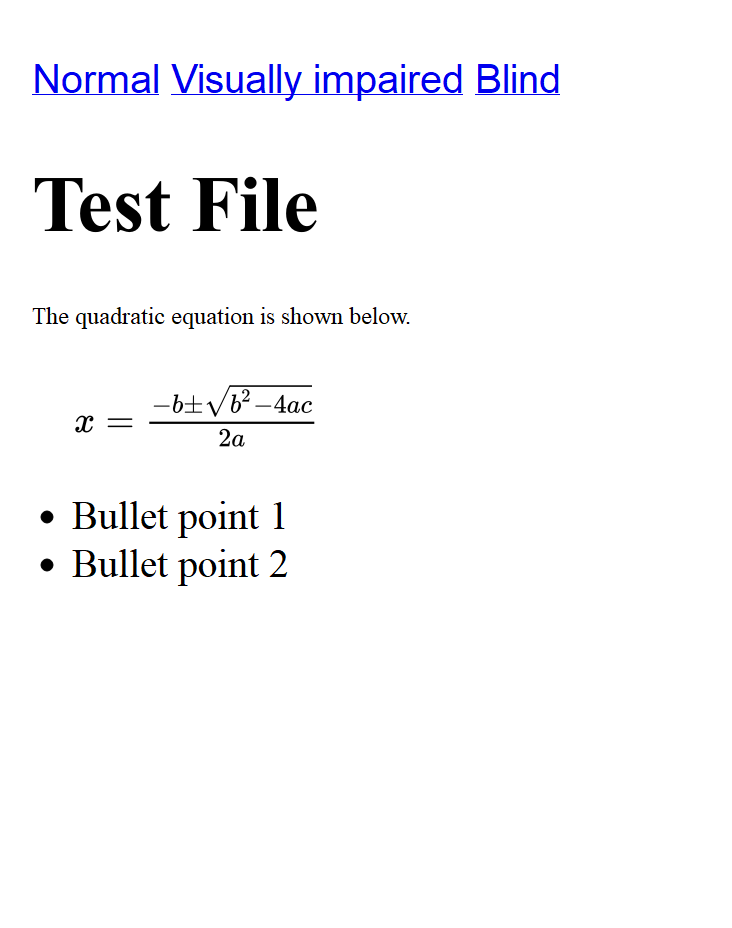
\includegraphics[height=10cm]{figures/ExampleEPUB1.png}}
	\end{minipage}\hfill
	\begin{minipage}{0.5\textwidth}
		\centering
		\fbox{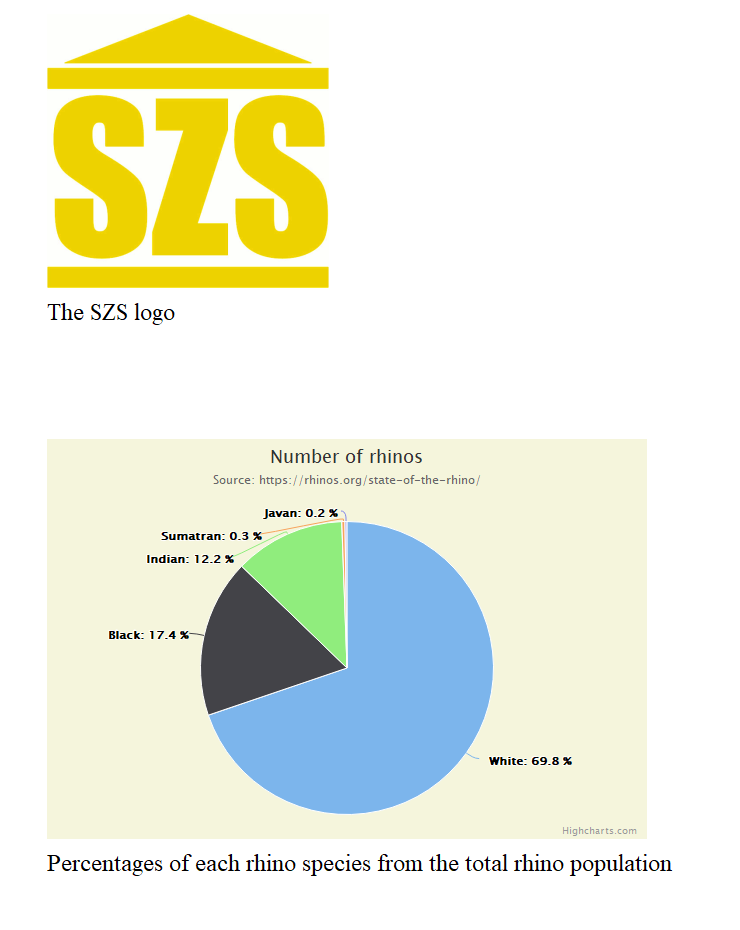
\includegraphics[height=10cm]{figures/ExampleEPUB2.png}}
	\end{minipage}

	\caption{Example EPUB which will be tested}
	\label{fig:exampleEPUB}
\end{figure}

This chapter is going to present an evaluation of how documents of the new standard were displayed in several EPUB reading systems. The test document has the same content that will be in both versions of the new standard. The CSS version is shown in figure \ref{fig:exampleEPUB}. It is shown in dual column mode so that the whole document can be shown at once. Actually the SZS logo is followed by the graph, so that is the proper reading order. The file has following content:

\begin{enumerate}
	\item A heading of level 1
	\item Standard text
	\item A figure with a MathML equation
	\item A short list
	\item A figure with a PNG
	\item A figure with a SVG
\end{enumerate}

All of these features are important to keep the document accessible. It is vital to have both a PNG and a SVG to test if a SVG can be displayed. Unlike PNG, they are not a standard format so they might not be supported. The operating systems tested are Android 8.1, iOS 11.2 and Windows 10.

\section{Reading systems on Android}
	
\subsection{Reasily}

\begin{figure}[h]
	
	\begin{minipage}{0.47\textwidth}
		\centering
		\fbox{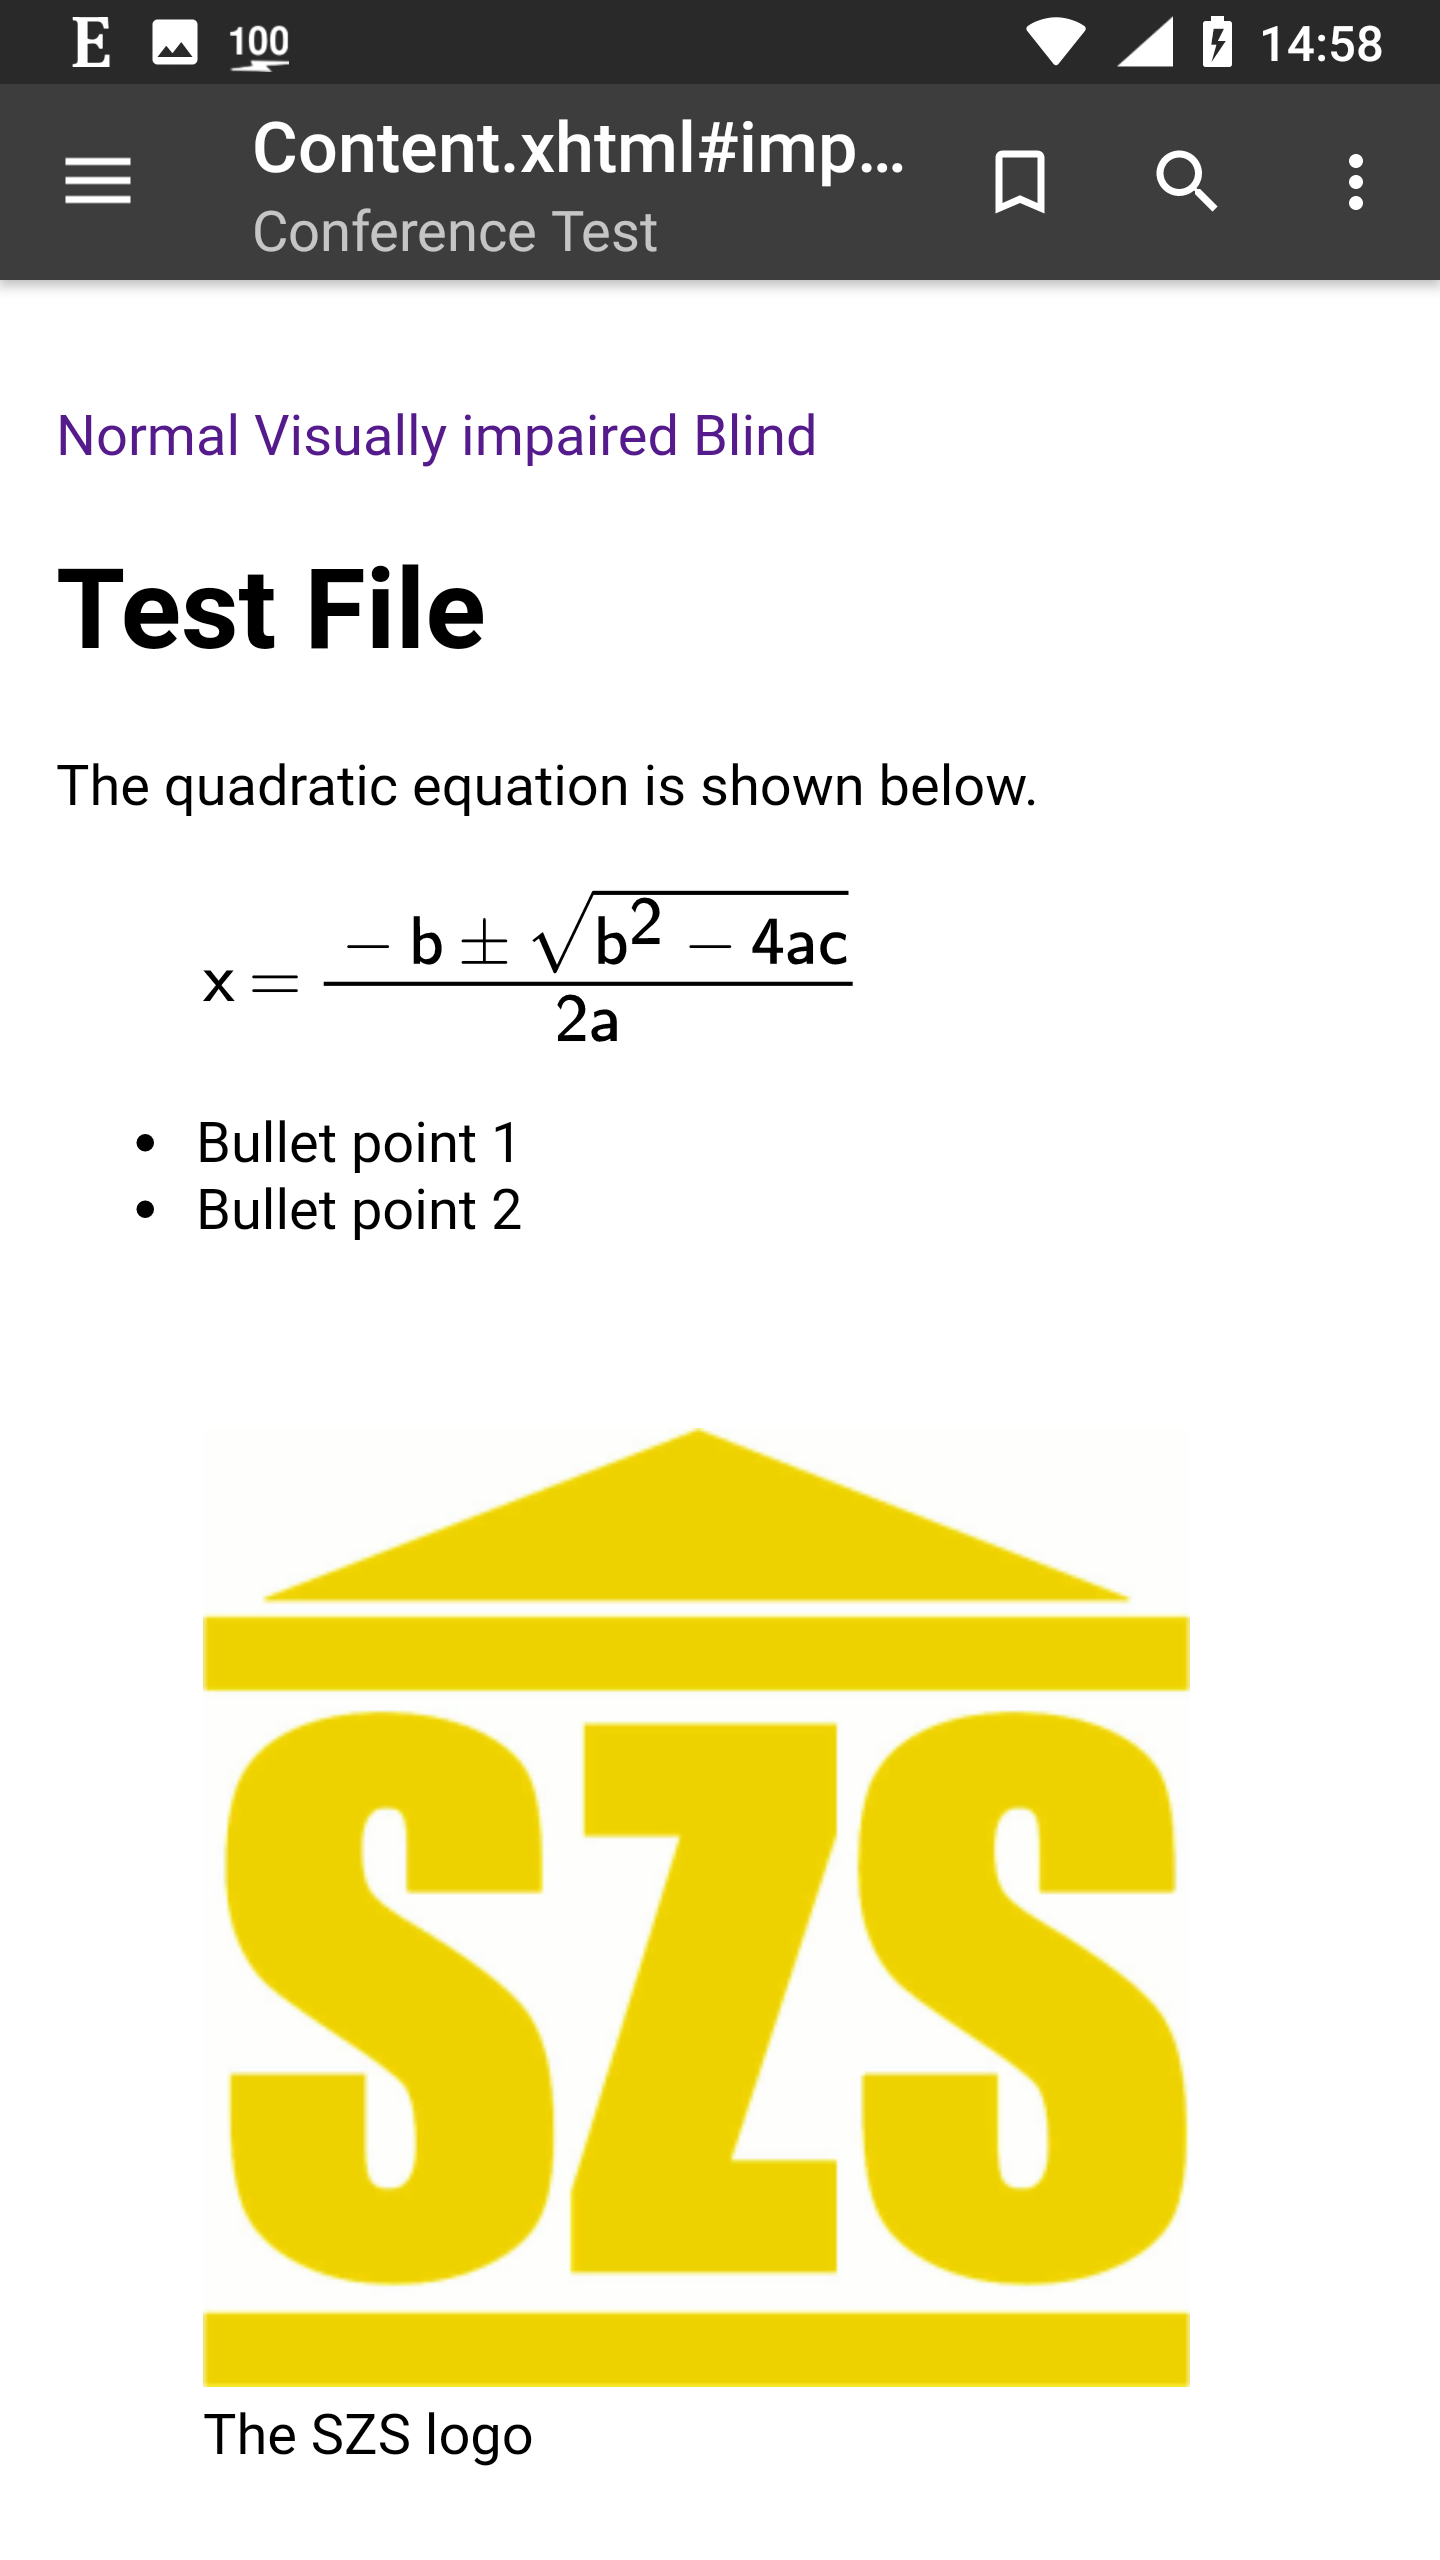
\includegraphics[width=\linewidth]{figures/ReasilyVi1.png}}
	\end{minipage}\hfill
	\hspace{0.05cm}
	\begin{minipage}{0.47\textwidth}
		\centering
		\fbox{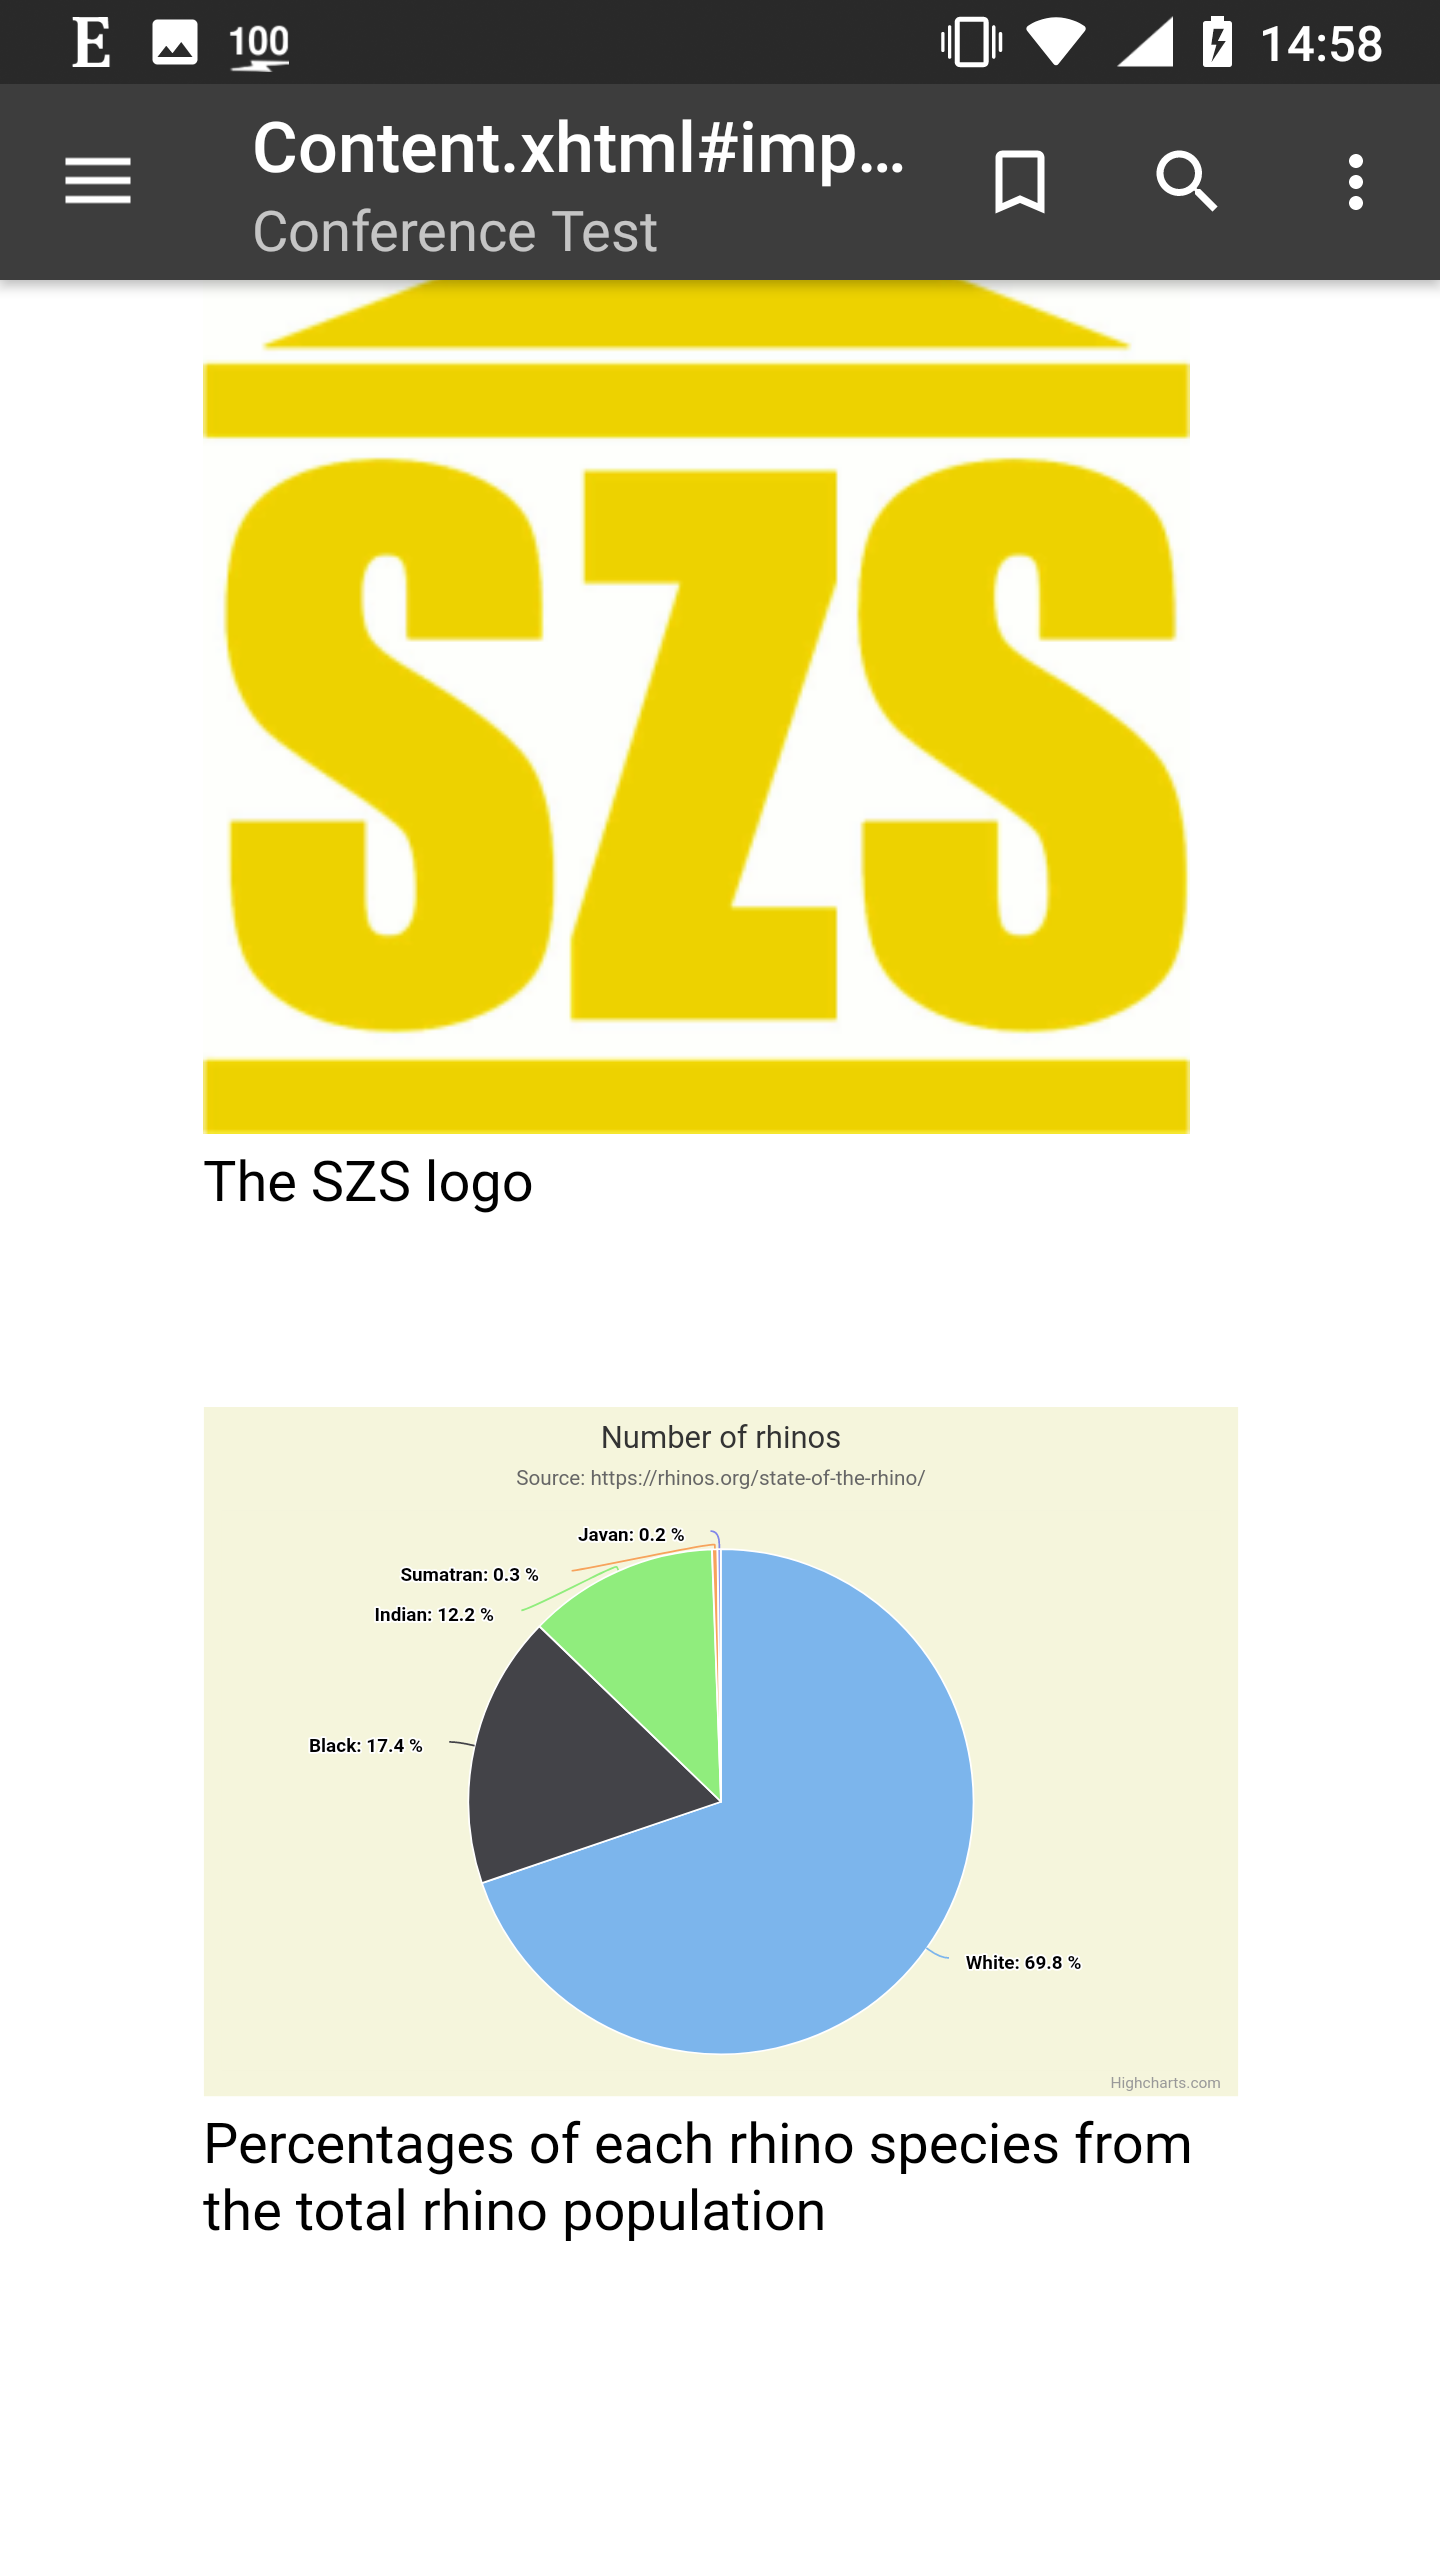
\includegraphics[width=\linewidth]{figures/ReasilyVi2.png}}
	\end{minipage}
	
	\caption{The visually impaired display style in Reasily}
	\label{fig:reasilyNo}
\end{figure}
Reasily is an Android EPUB reading app which states that it has support for several EPUB 3 features such as MathML and media overlay for read aloud books\footnote{https://play.google.com/store/apps/details?id=com.gmail.jxlab.app.reasily}. While the JavaScript standard does not switch versions correctly, the CSS version does. The normal display style is shown in figure \ref{fig:reasilyNo}. All elements are shown as desired. Each of the figures with MathML, PNG and SVG are displayed properly. 

\begin{comment}
\begin{figure}[h]
	\begin{minipage}{0.5\textwidth}
		\centering
		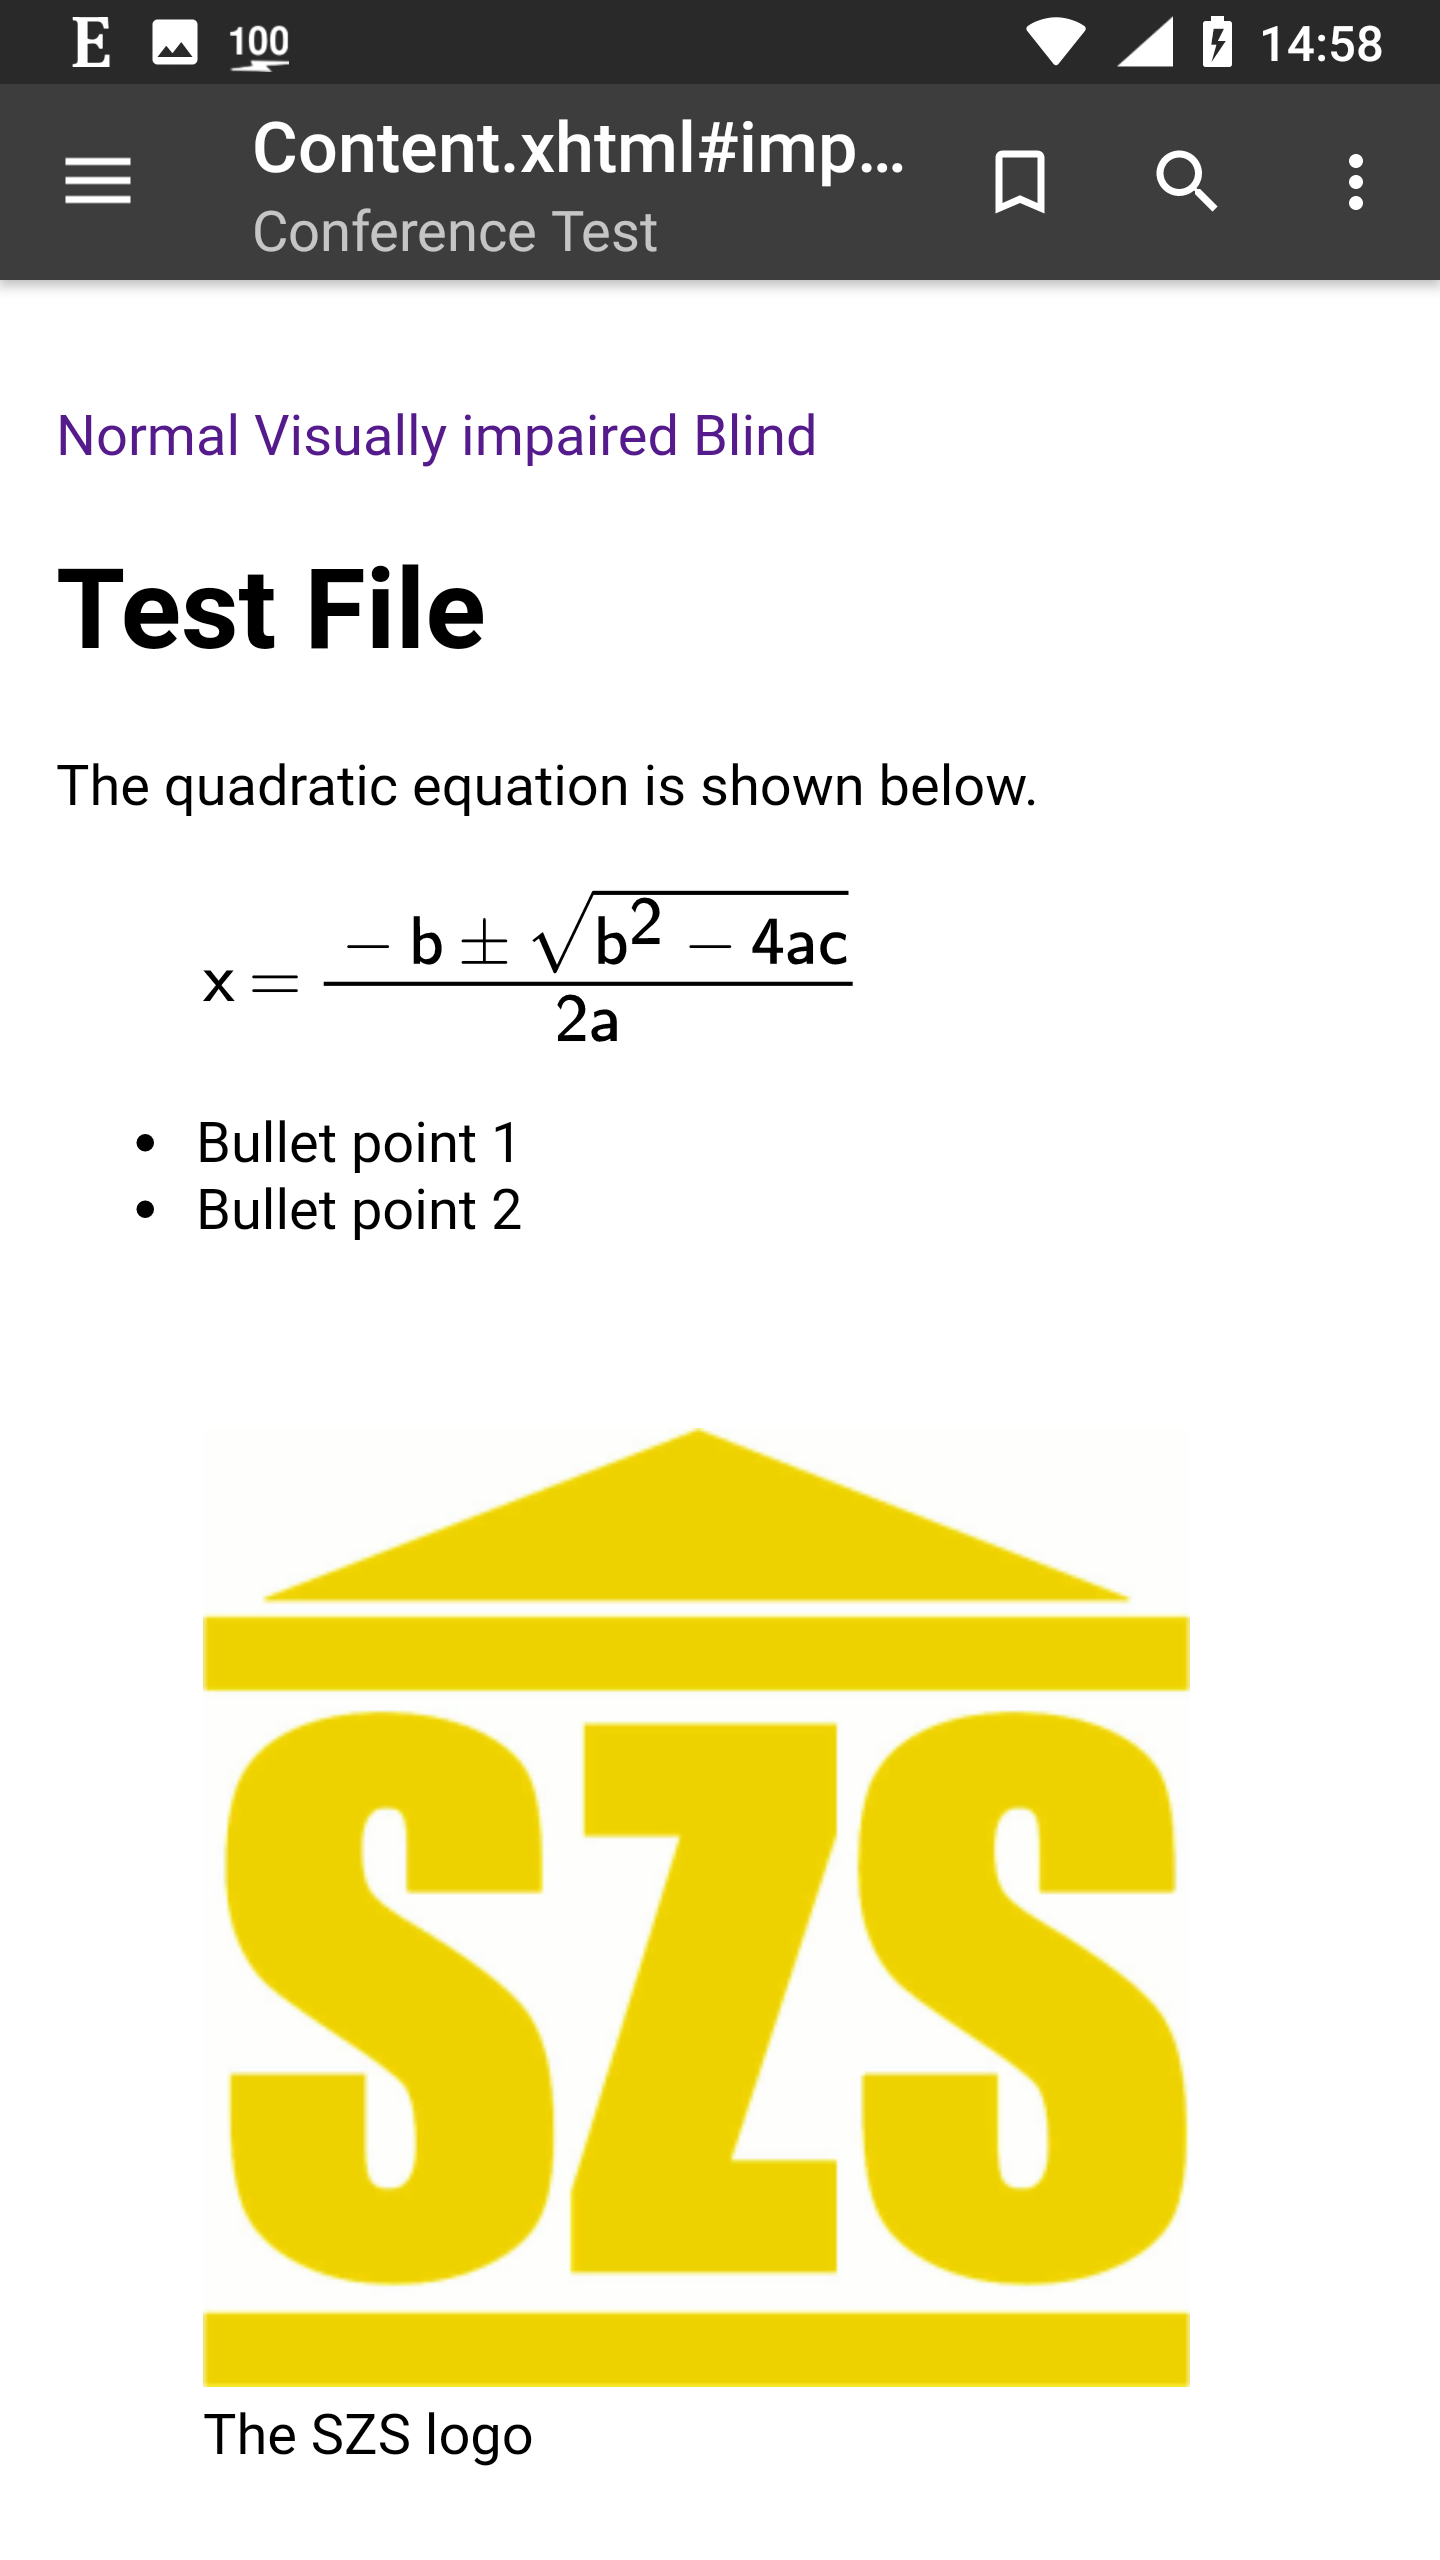
\includegraphics[width=\linewidth]{figures/ReasilyVi1.png}
	\end{minipage}\hfill
	\begin{minipage}{0.5\textwidth}
		\centering
		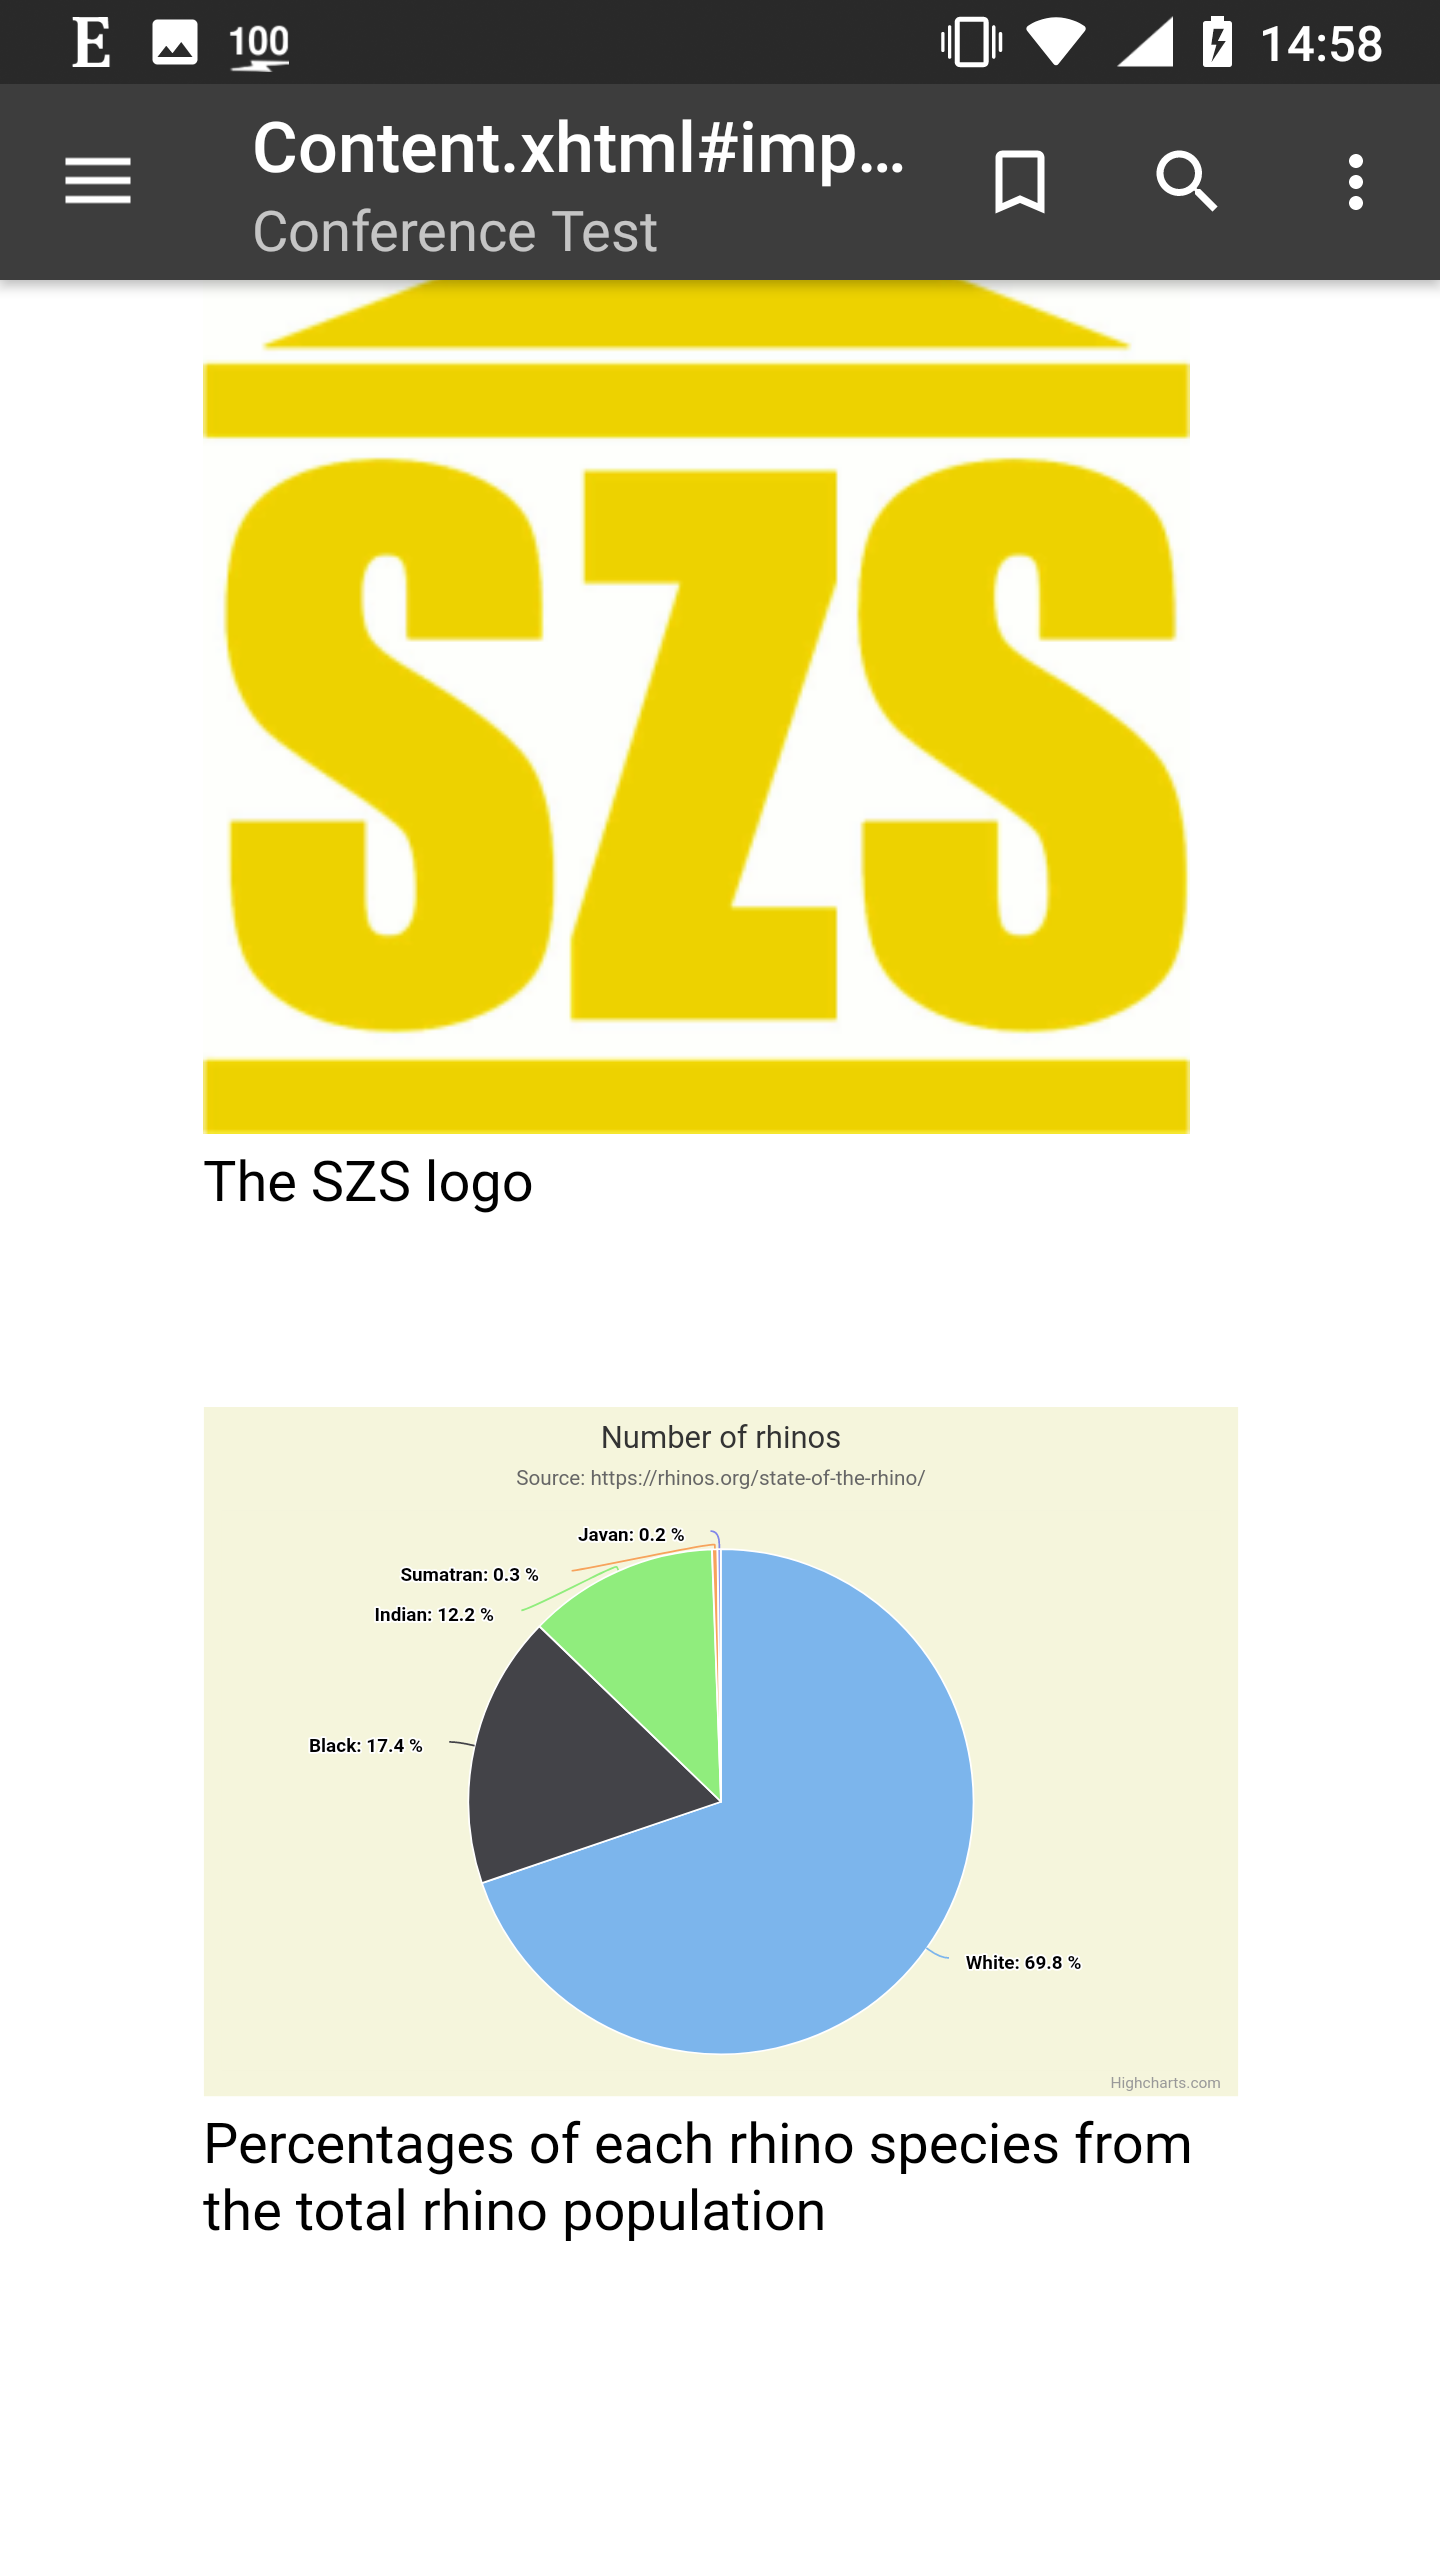
\includegraphics[width=\linewidth]{figures/ReasilyVi2.png}
	\end{minipage}
	\caption{The visually impaired display style in Reasily}
	\label{fig:reasilyVi}
\end{figure}
\end{comment}

The visually impaired display style is also shown properly, with the MathML equation using a sans serif font. The blind display style in figure \ref{fig:reasilyBl} is shown correctly, with the equations and images showing the alternative text with the appropriate tags. Furthermore, Reasily supports TalkBack and elements such as the heading of level 1 are identified properly.

\begin{figure}[H]
	\centering
	\fbox{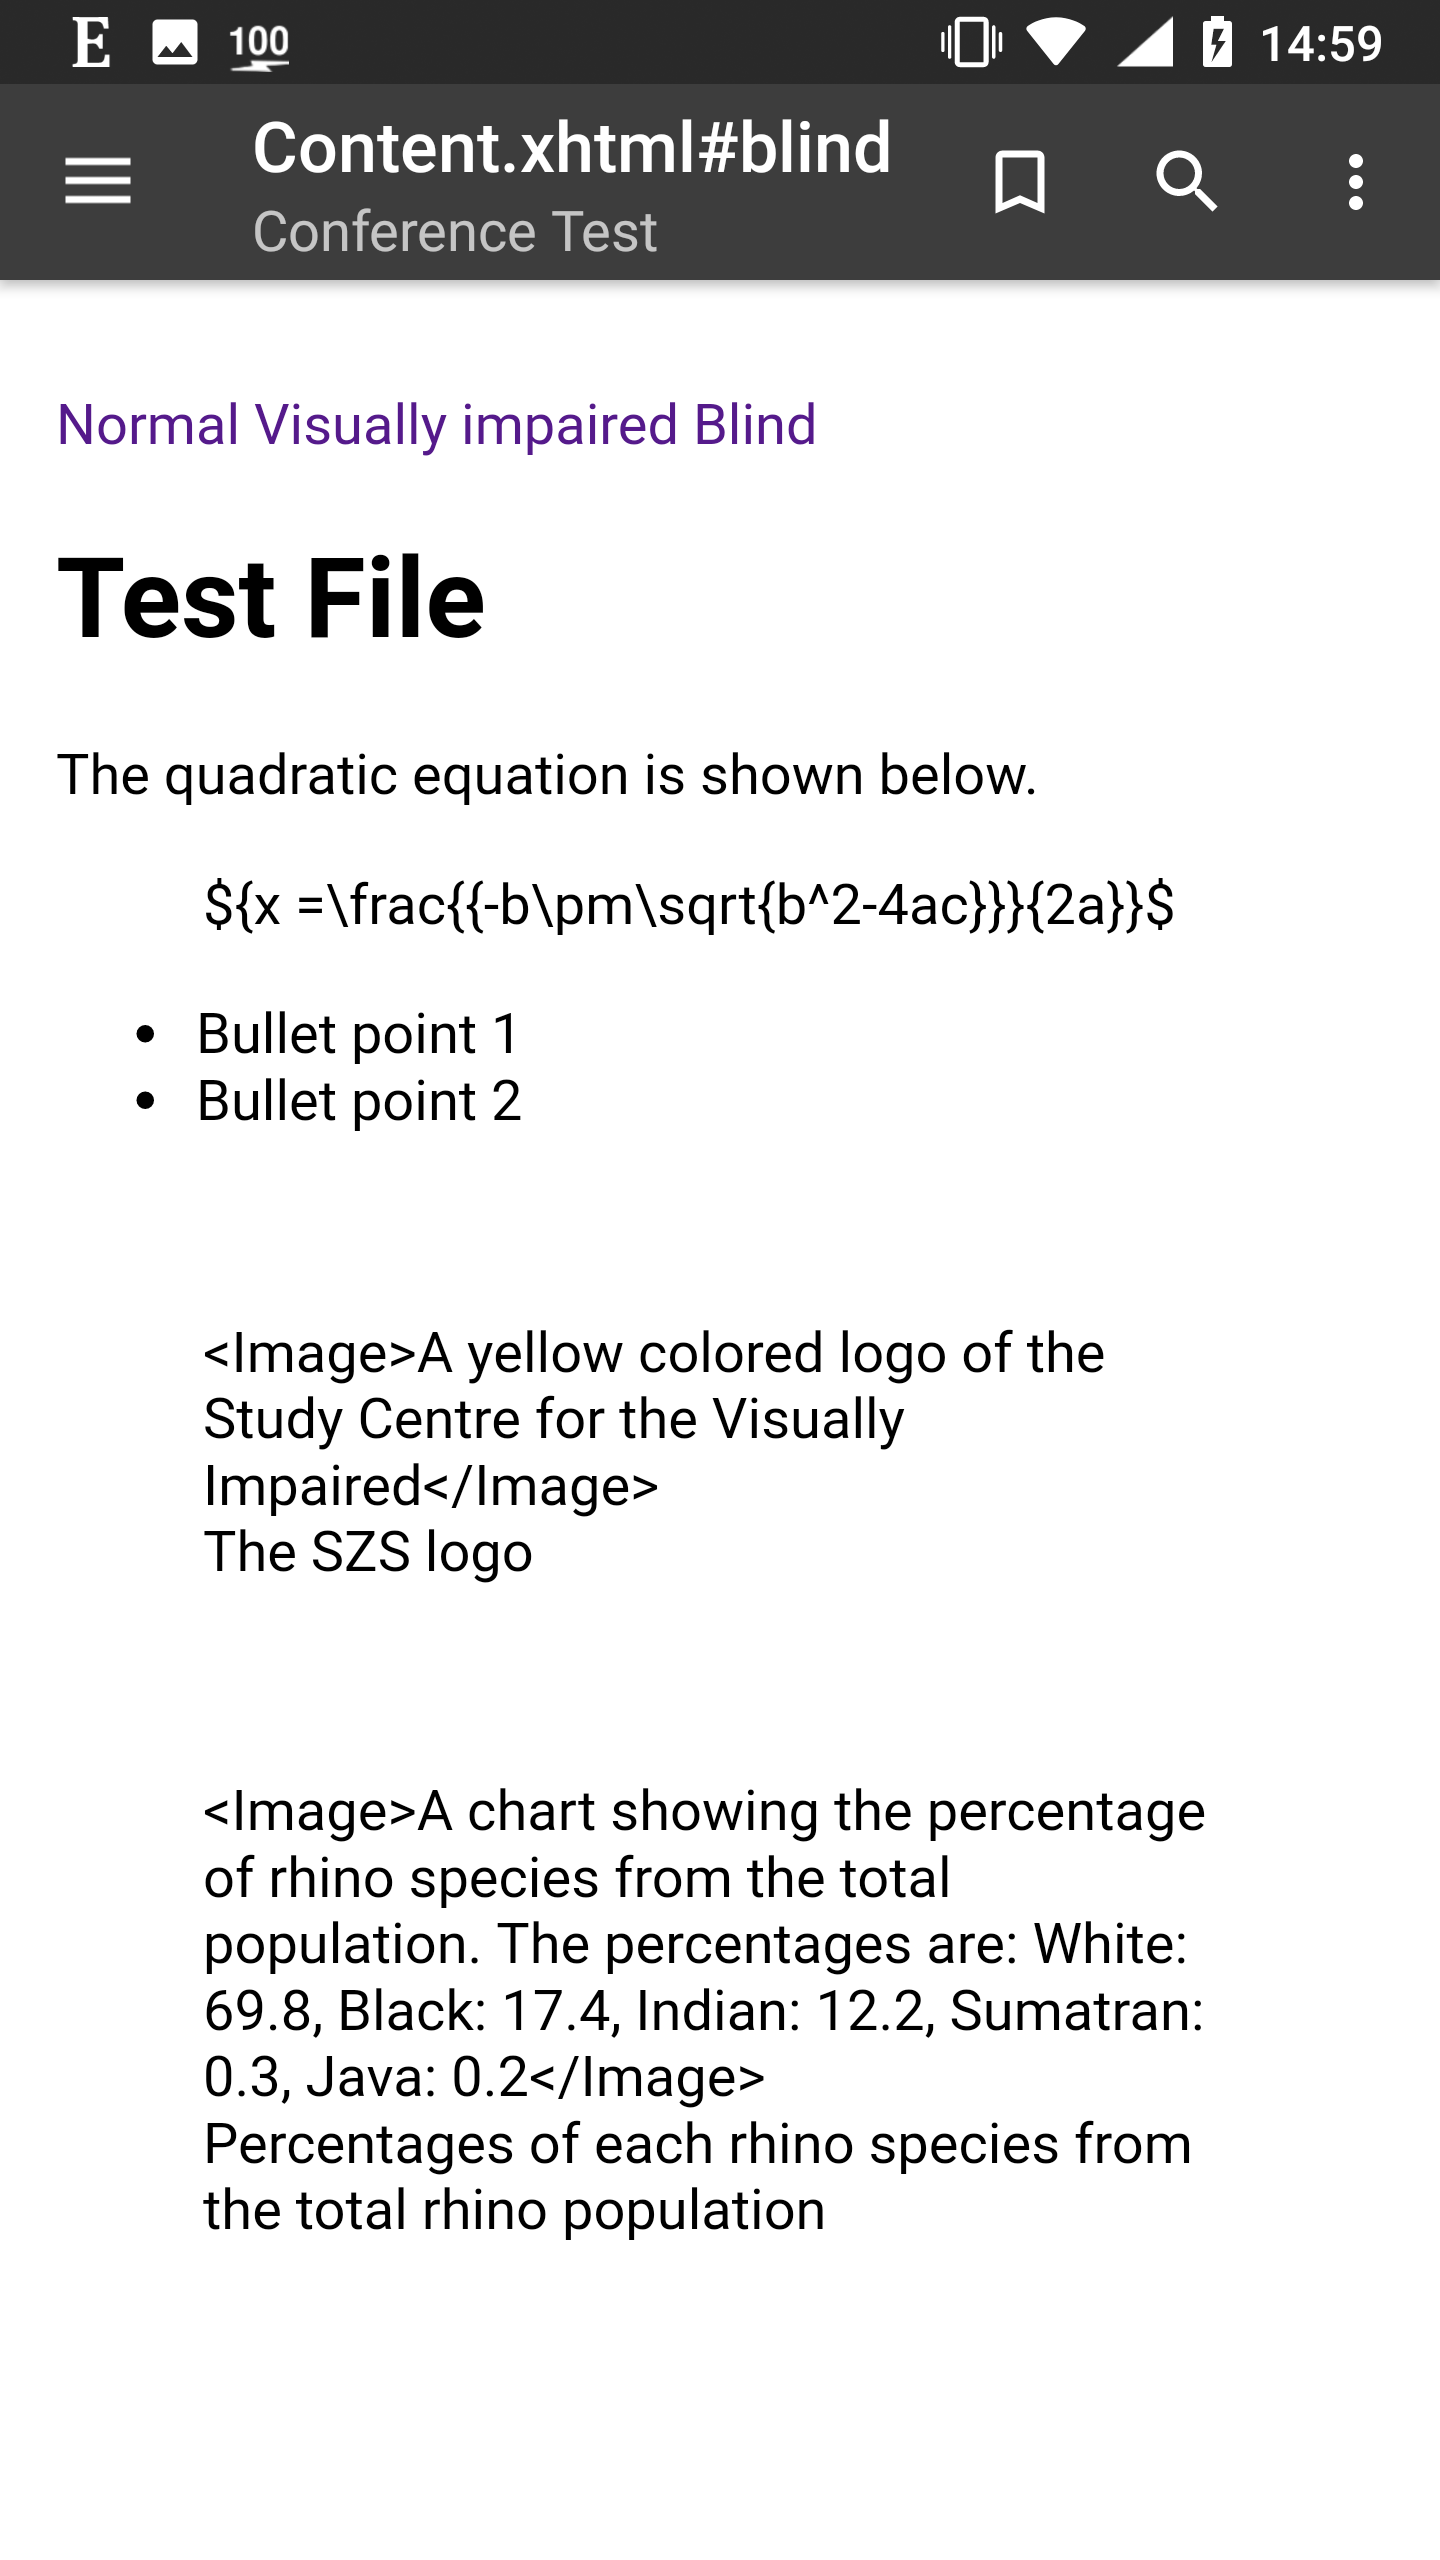
\includegraphics[width=\linewidth/3]{figures/ReasilyBl.png}}
	\caption{The blind display style in Reasily}
	\label{fig:reasilyBl}
\end{figure}

\subsection{Unusable reading systems}

\subsubsection{Tolino}
Tolino is a cooperation of several large German booksellers to create a unified E-Book reading device\footnote{https://mytolino.de/tolino-kooperationen-und-vertrieb/}. There is a Tolino app on Android which can be used to see how well the EPUBs following the document standard run on the Tolino reading device family, as they likely share similar technology. However, the Android app is more powerful than the Tolino reading devices as it can also show color beyond greyscale. As seen in figure \ref{fig:tolino}, the app is unable to display MathML. Furthermore, it does not show the PNG file, which should actually be supported, as other files with images are displayed properly. This is due to the image being enclosed in a figure element. If it is not in one, the image is displayed correctly. 

\begin{figure}[h]
	\centering
	\fbox{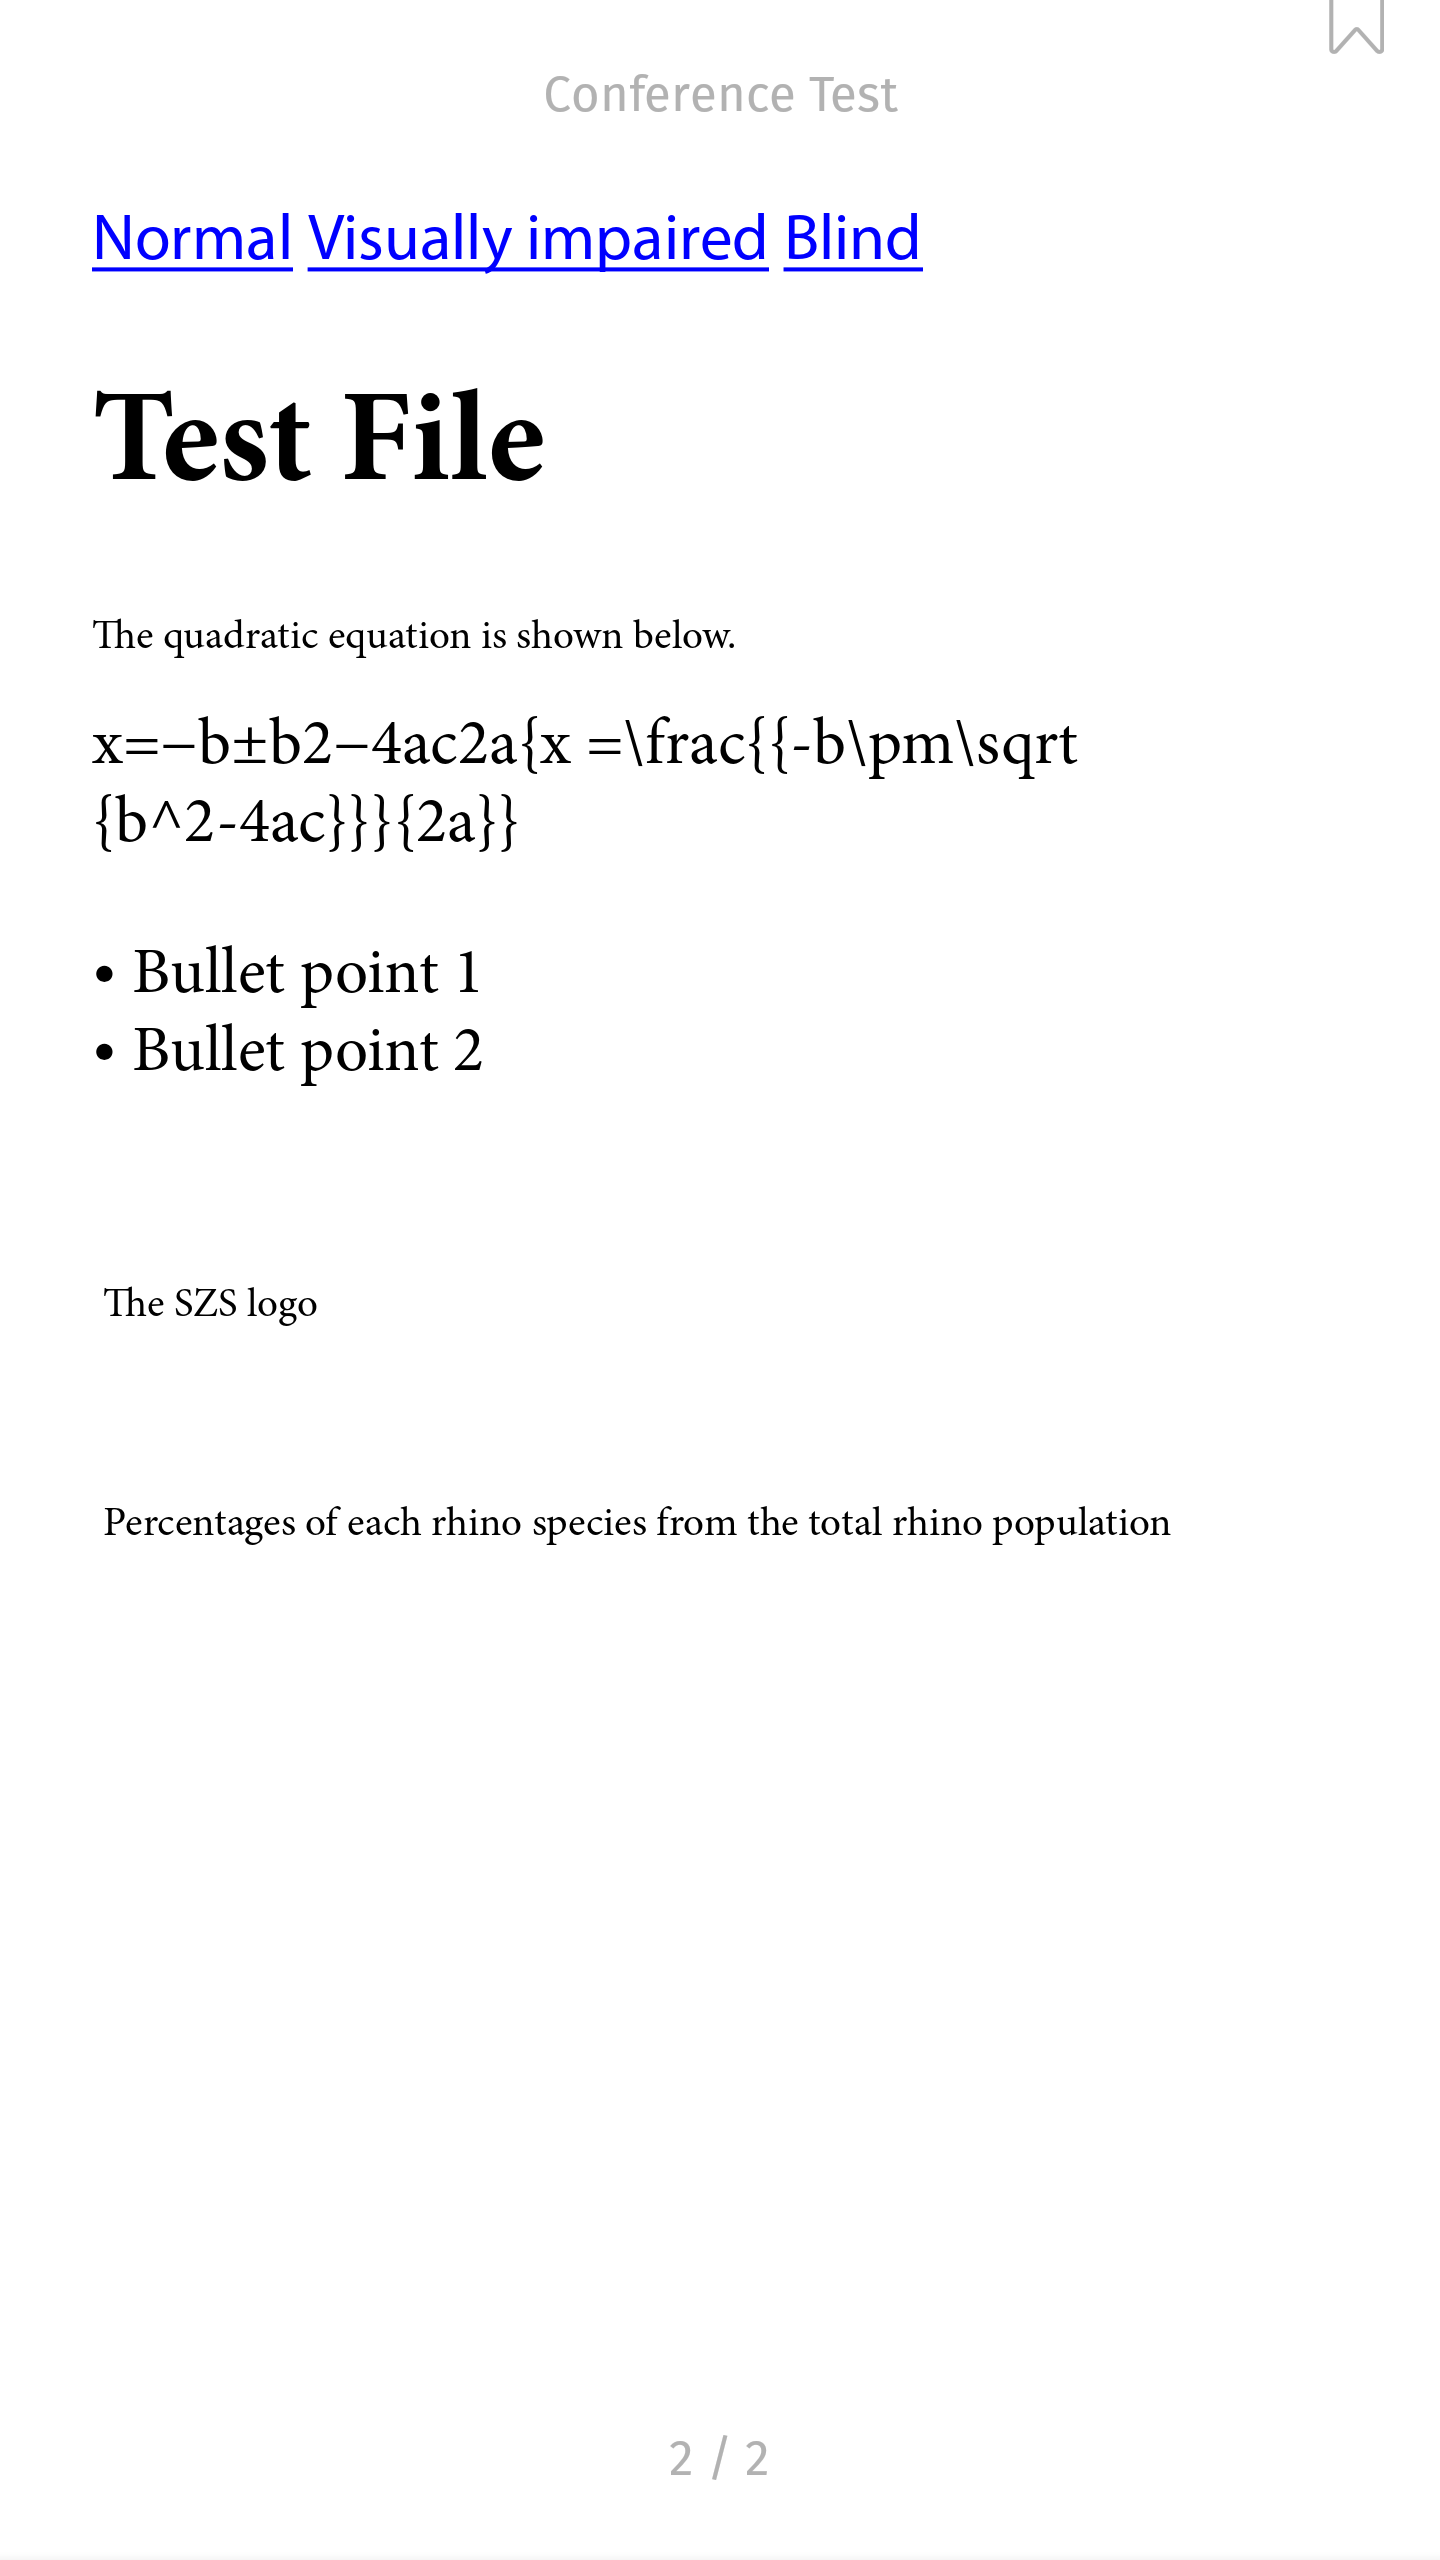
\includegraphics[width=\linewidth/3]{figures/Tolino.png}}
	\caption{EPUB of the CSS standard shown in Tolino}
	\label{fig:tolino}
\end{figure}

The switching mechanism does not work with both the CSS and JavaScript versions. This means that the Tolino app does not support scripting and also does  not support CSS 3. The preinstalled screen reader of Android, TalkBack, also does not work with the Tolino app.

\subsubsection{Gitden Reader}

Gitden Reader is an Android app\footnote{https://play.google.com/store/apps/details?id=com.gitden.epub.reader.app} with MathML support. It does not support both of the switching mechanisms, but does display the MathML, PNG and SVG properly. It supports TalkBack, but the equation is not identified properly and not read aloud.

\subsubsection{FBReader}
\begin{figure}[H]
	\centering
	\fbox{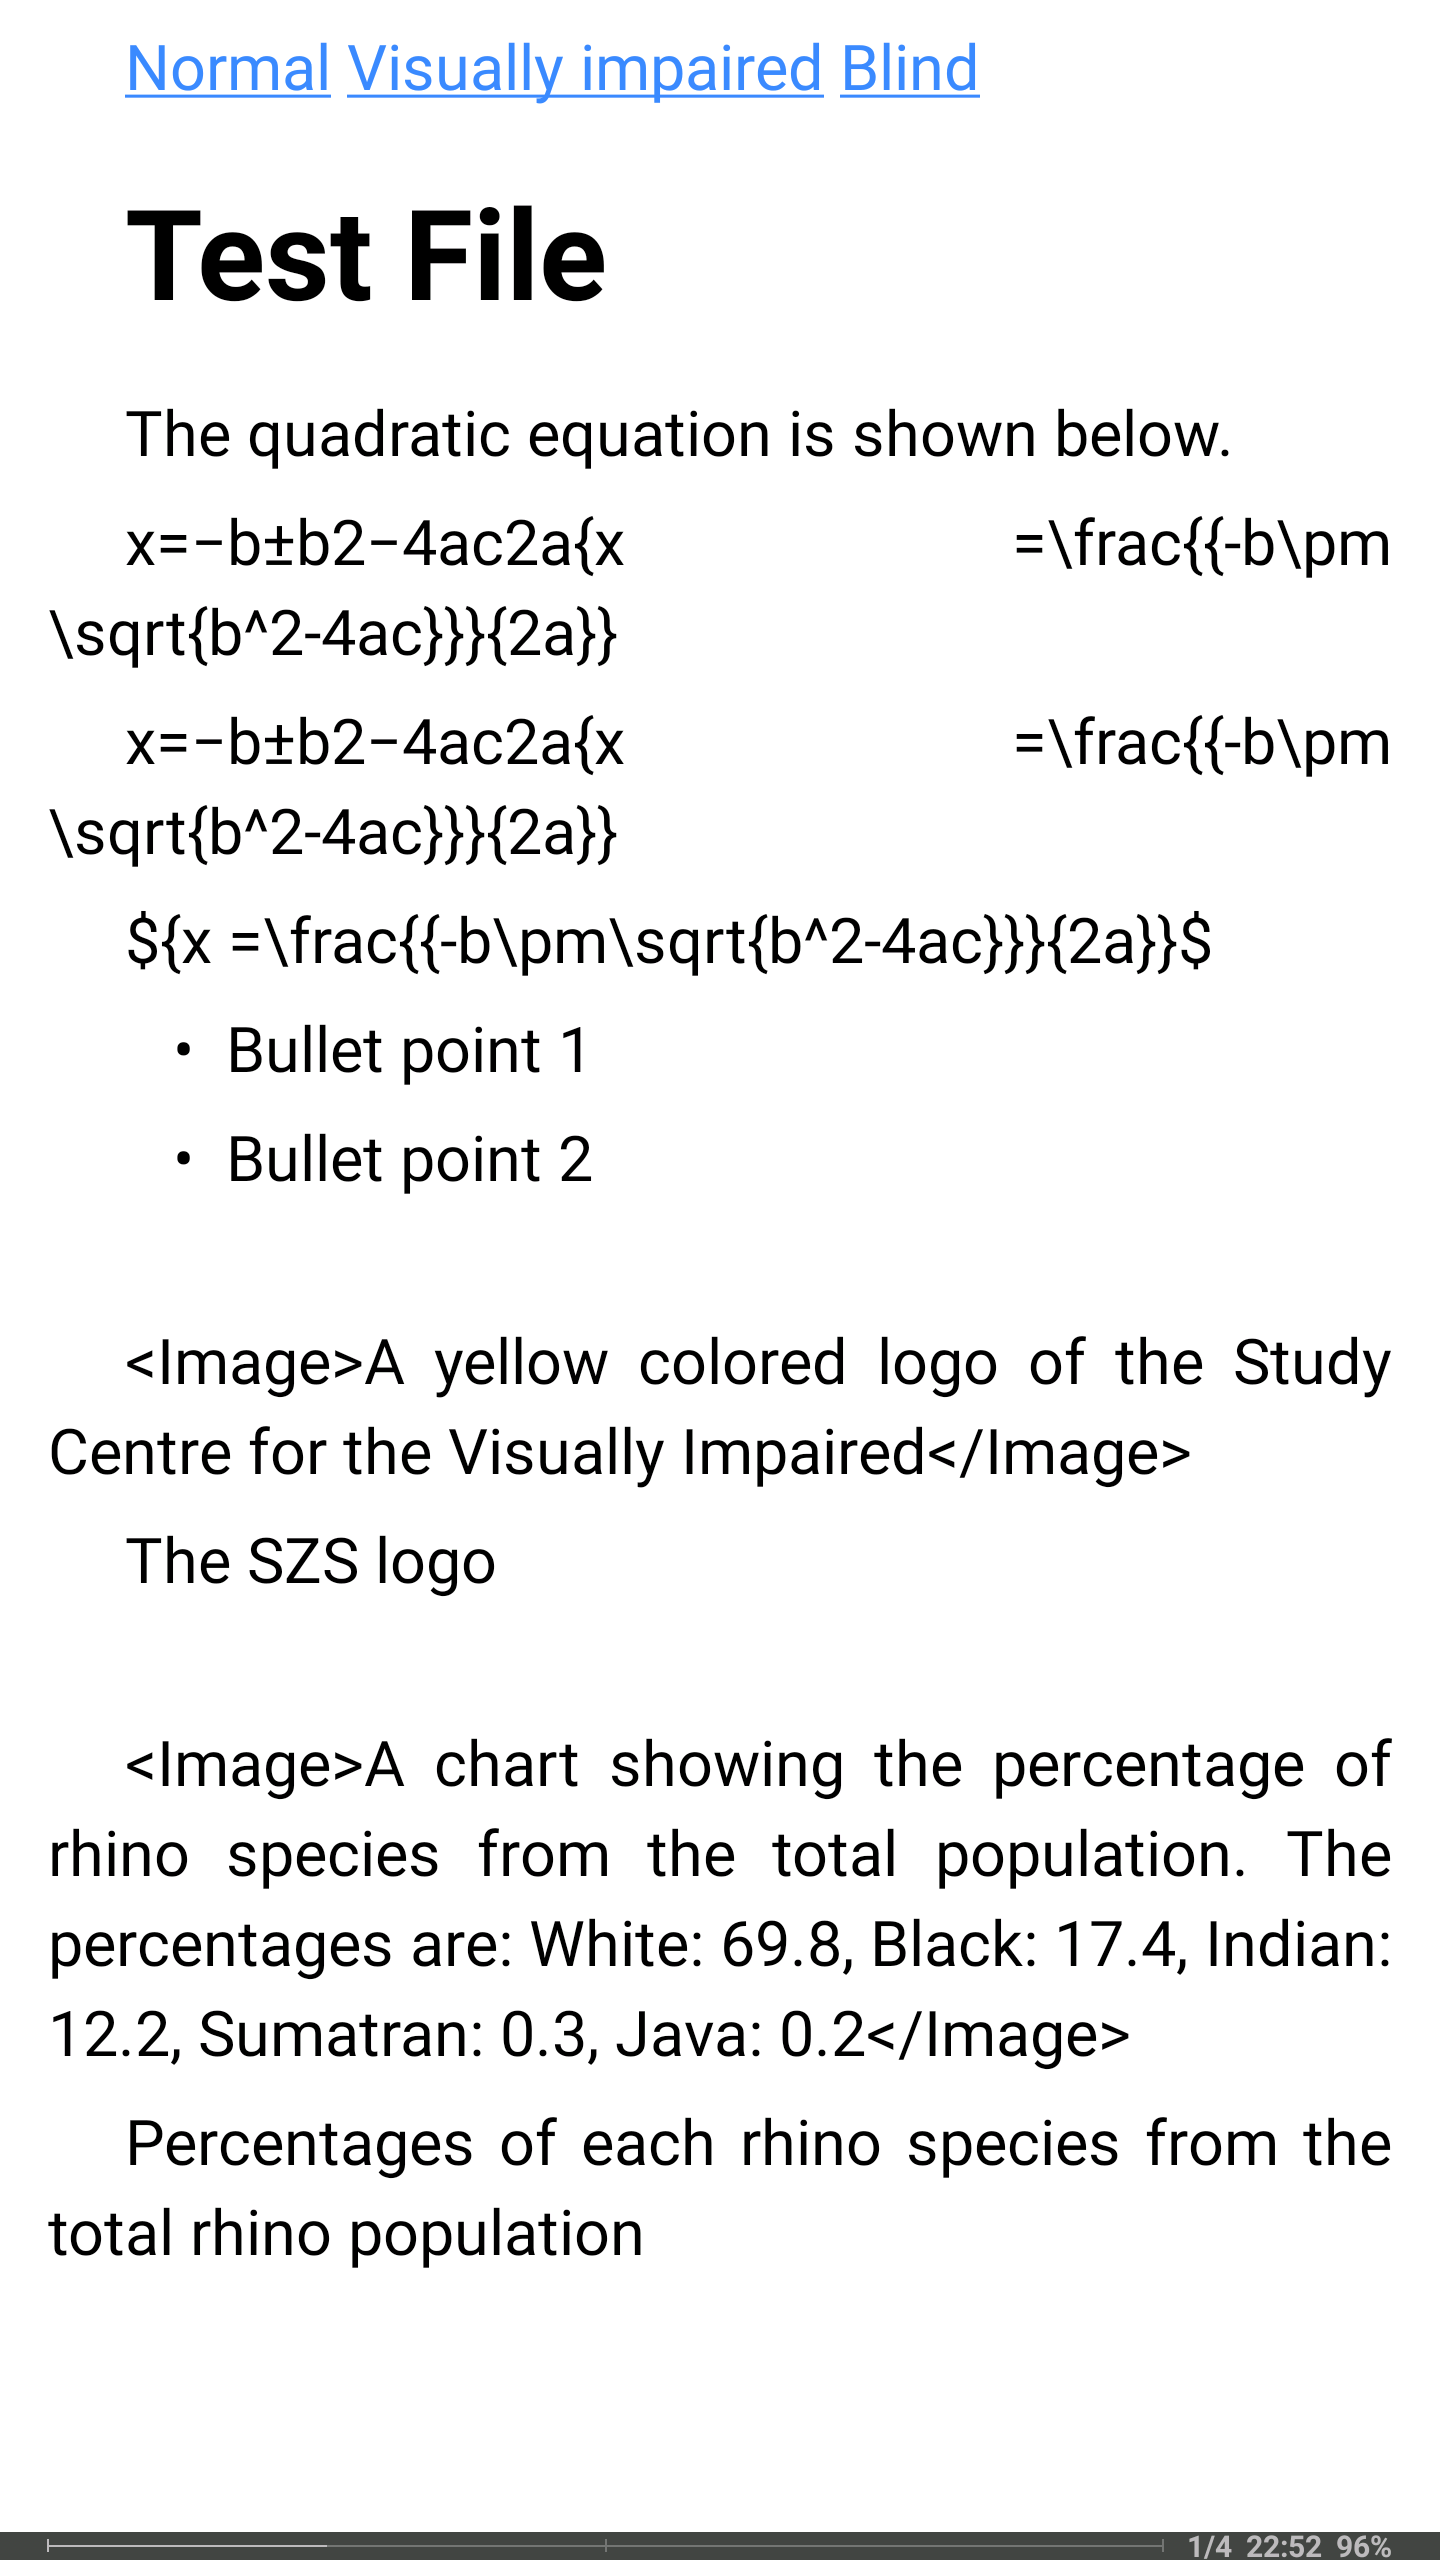
\includegraphics[width=\linewidth/3]{figures/fbreader.png}}
	\caption{The CSS file in FBReader}
	\label{fig:fbreader}
\end{figure}
FBReader is a popular E-Book reader available on Android\footnote{https://play.google.com/store/apps/details?id=org.geometerplus.zlibrary.ui.android}. Both CSS and JavaScript switching do not function as intended. Furthermore, none of the MathML, PNG and SVG are shown properly. The MathML first shows the equation not rendered properly and then annotation which should actually be hidden. One interesting observation is that elements which are supposed to be hidden, such as the text between the \lstinline|<Image>| tags, are shown. The CSS file even has three pages showing the same page as shown in figure \ref{fig:fbreader}, only the links at the top are missing. Thus it is likely that FBReader does not support certain CSS features such as hiding elements.

\subsubsection{UB Reader}

\begin{figure}[H]
	\centering
	\fbox{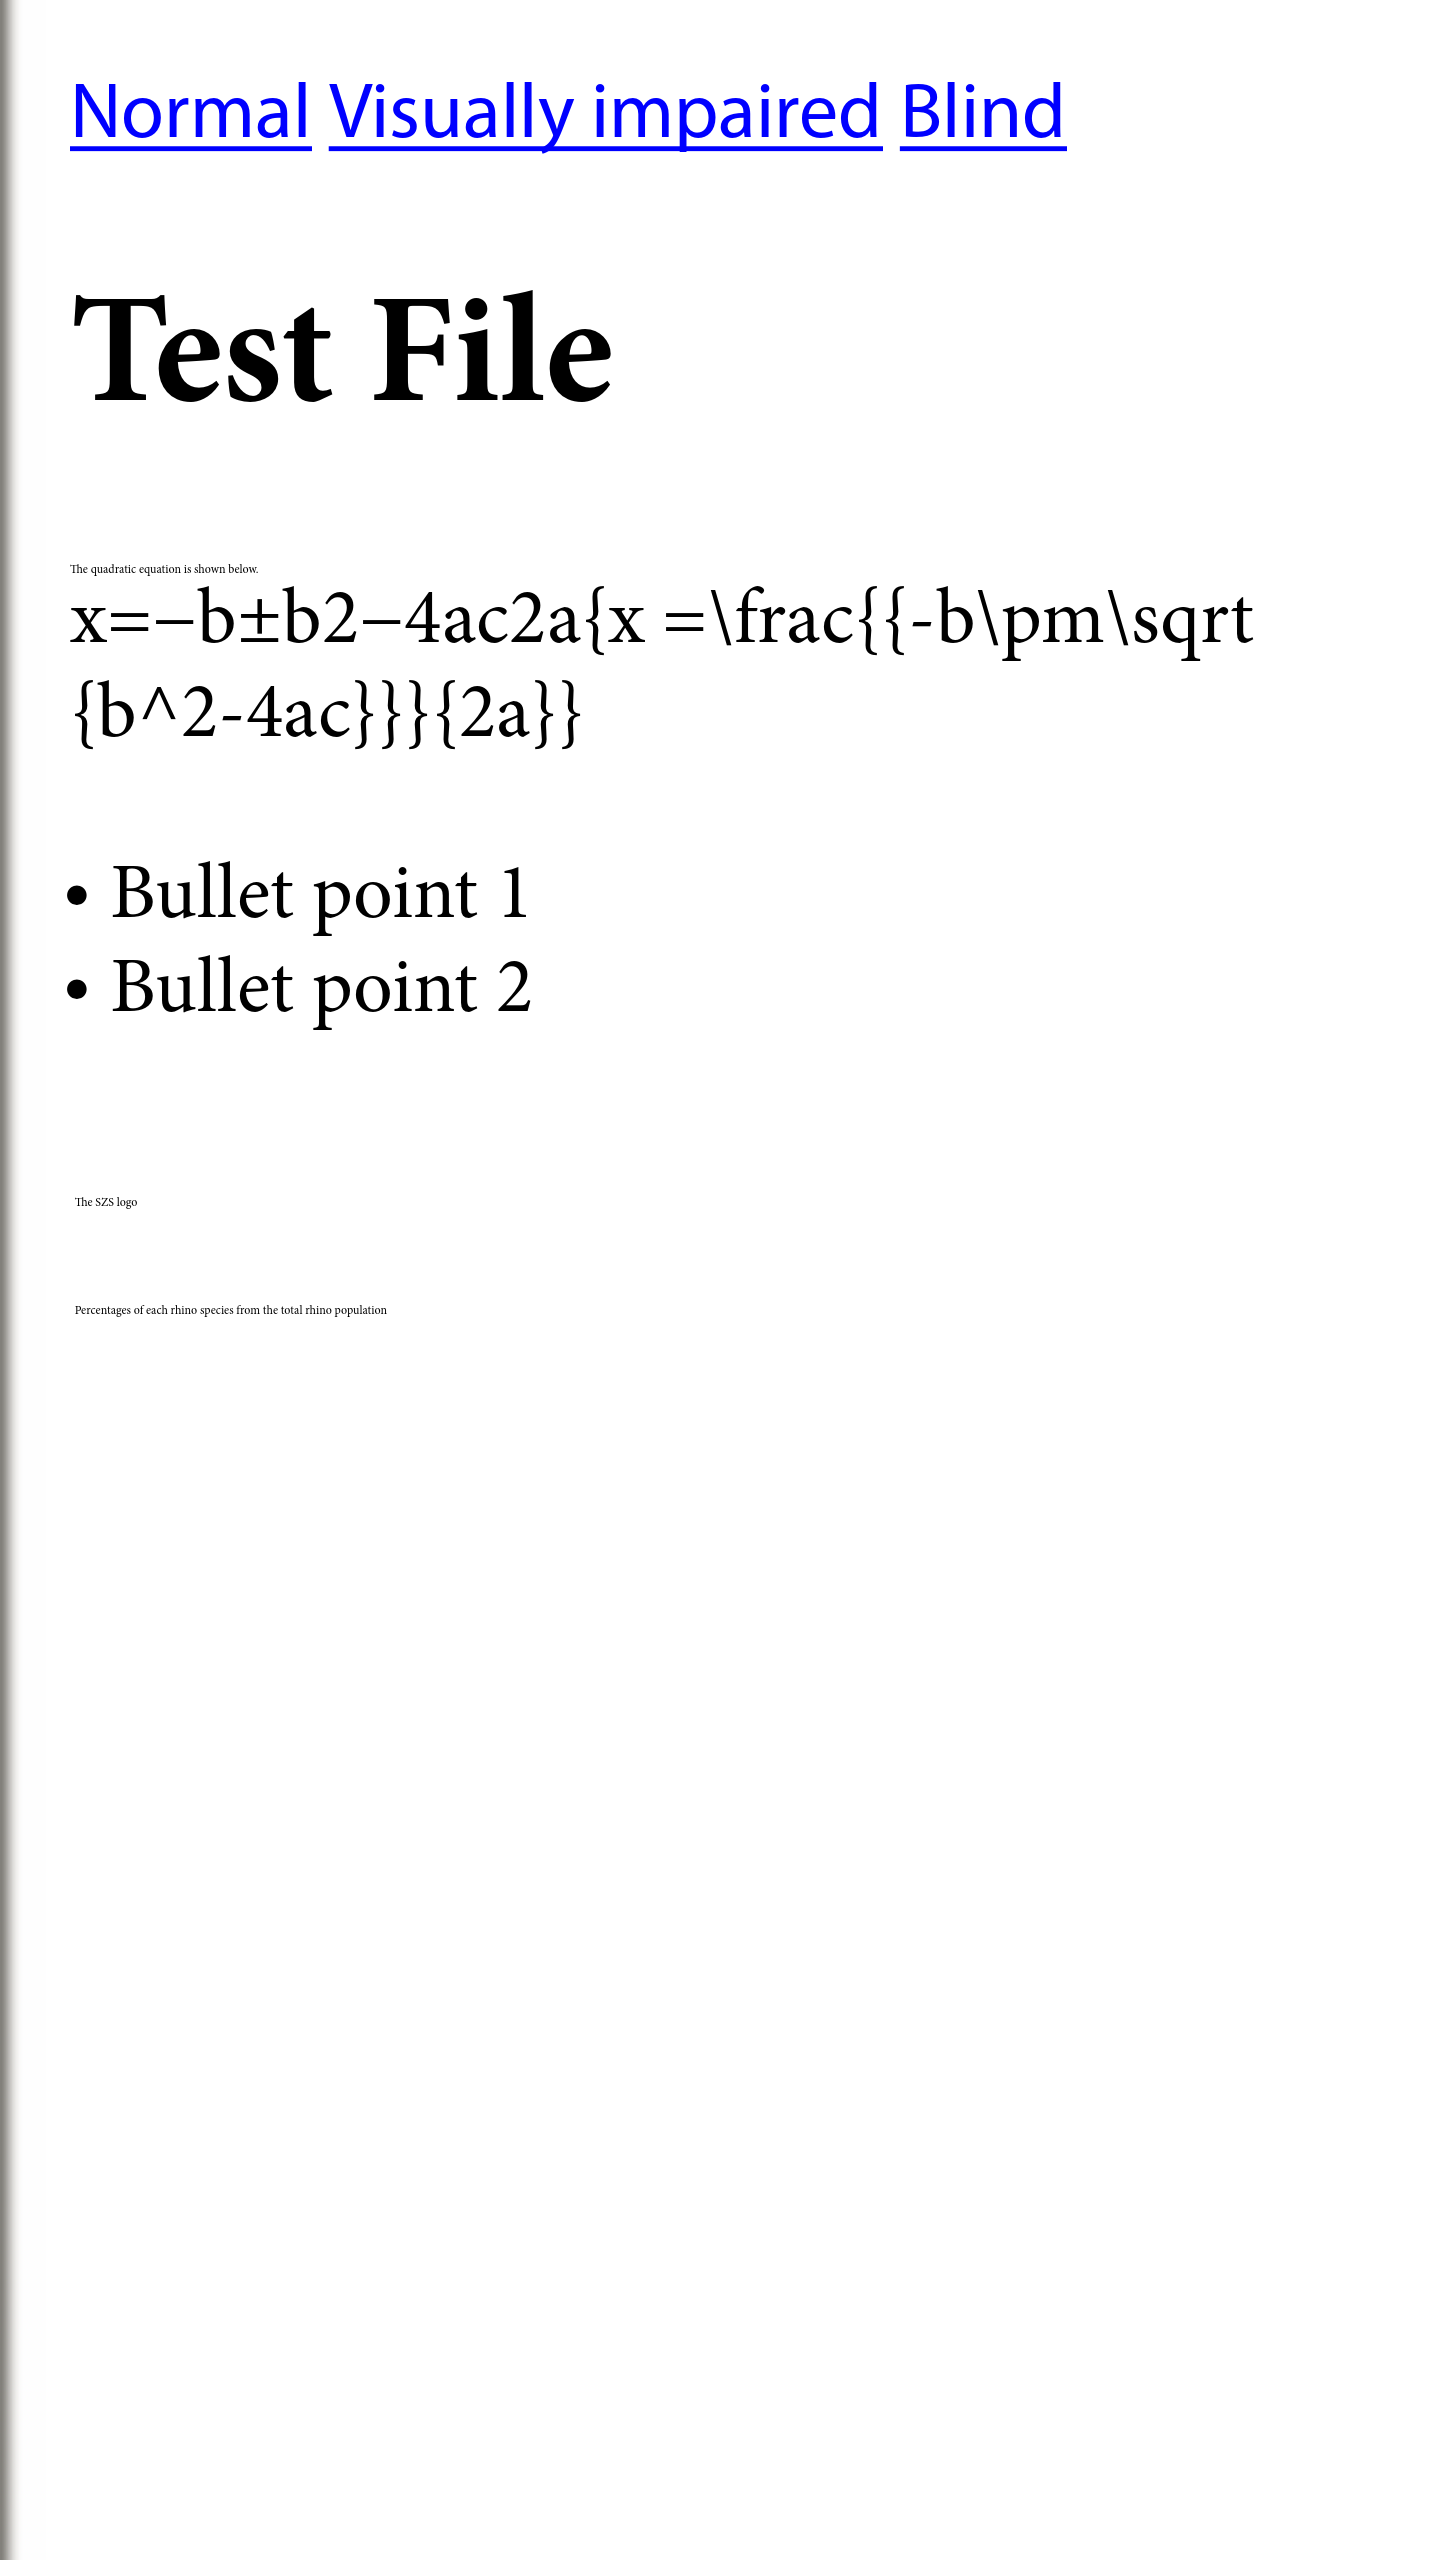
\includegraphics[width=\linewidth/3]{figures/ubreader.png}}
	\caption{The CSS file in UB Reader}
	\label{fig:ubreader}
\end{figure}
UB Reader (Universal Book Reader) is another popular Android E-Book reader\footnote{https://play.google.com/store/apps/details?id=com.mobisystems.ubreader\_west}. The switching mechanism does not work with either standard and as shown in figure \ref{fig:ubreader}, the equation and the images are not shown. Strangely enough, the standard text is shown very small, while links, bullet points and other text is shown much larger.

\section{Reading systems on iOS}
\subsection{Marvin}


Marvin is an app for iOS devices\footnote{https://itunes.apple.com/app/id1086482858} and the JavaScript version is displayed correctly. The CSS version does not work.It also renders the SVG correctly, but it is not in the figure. The only problem is with the script size in the visually impaired display style in \ref{fig:marvinVi}. The exponent of b should be the same size like in Reasily shown in figure \ref{fig:reasilyVi}. This will have to be tested further. The blind display style is shown correctly, much like in figure \ref{fig:reasilyBl}. The iOS screen reader, VoiceOver, works very well in Marvin, identifying all elements correctly.

\begin{figure}[H]
	\centering
	\fbox{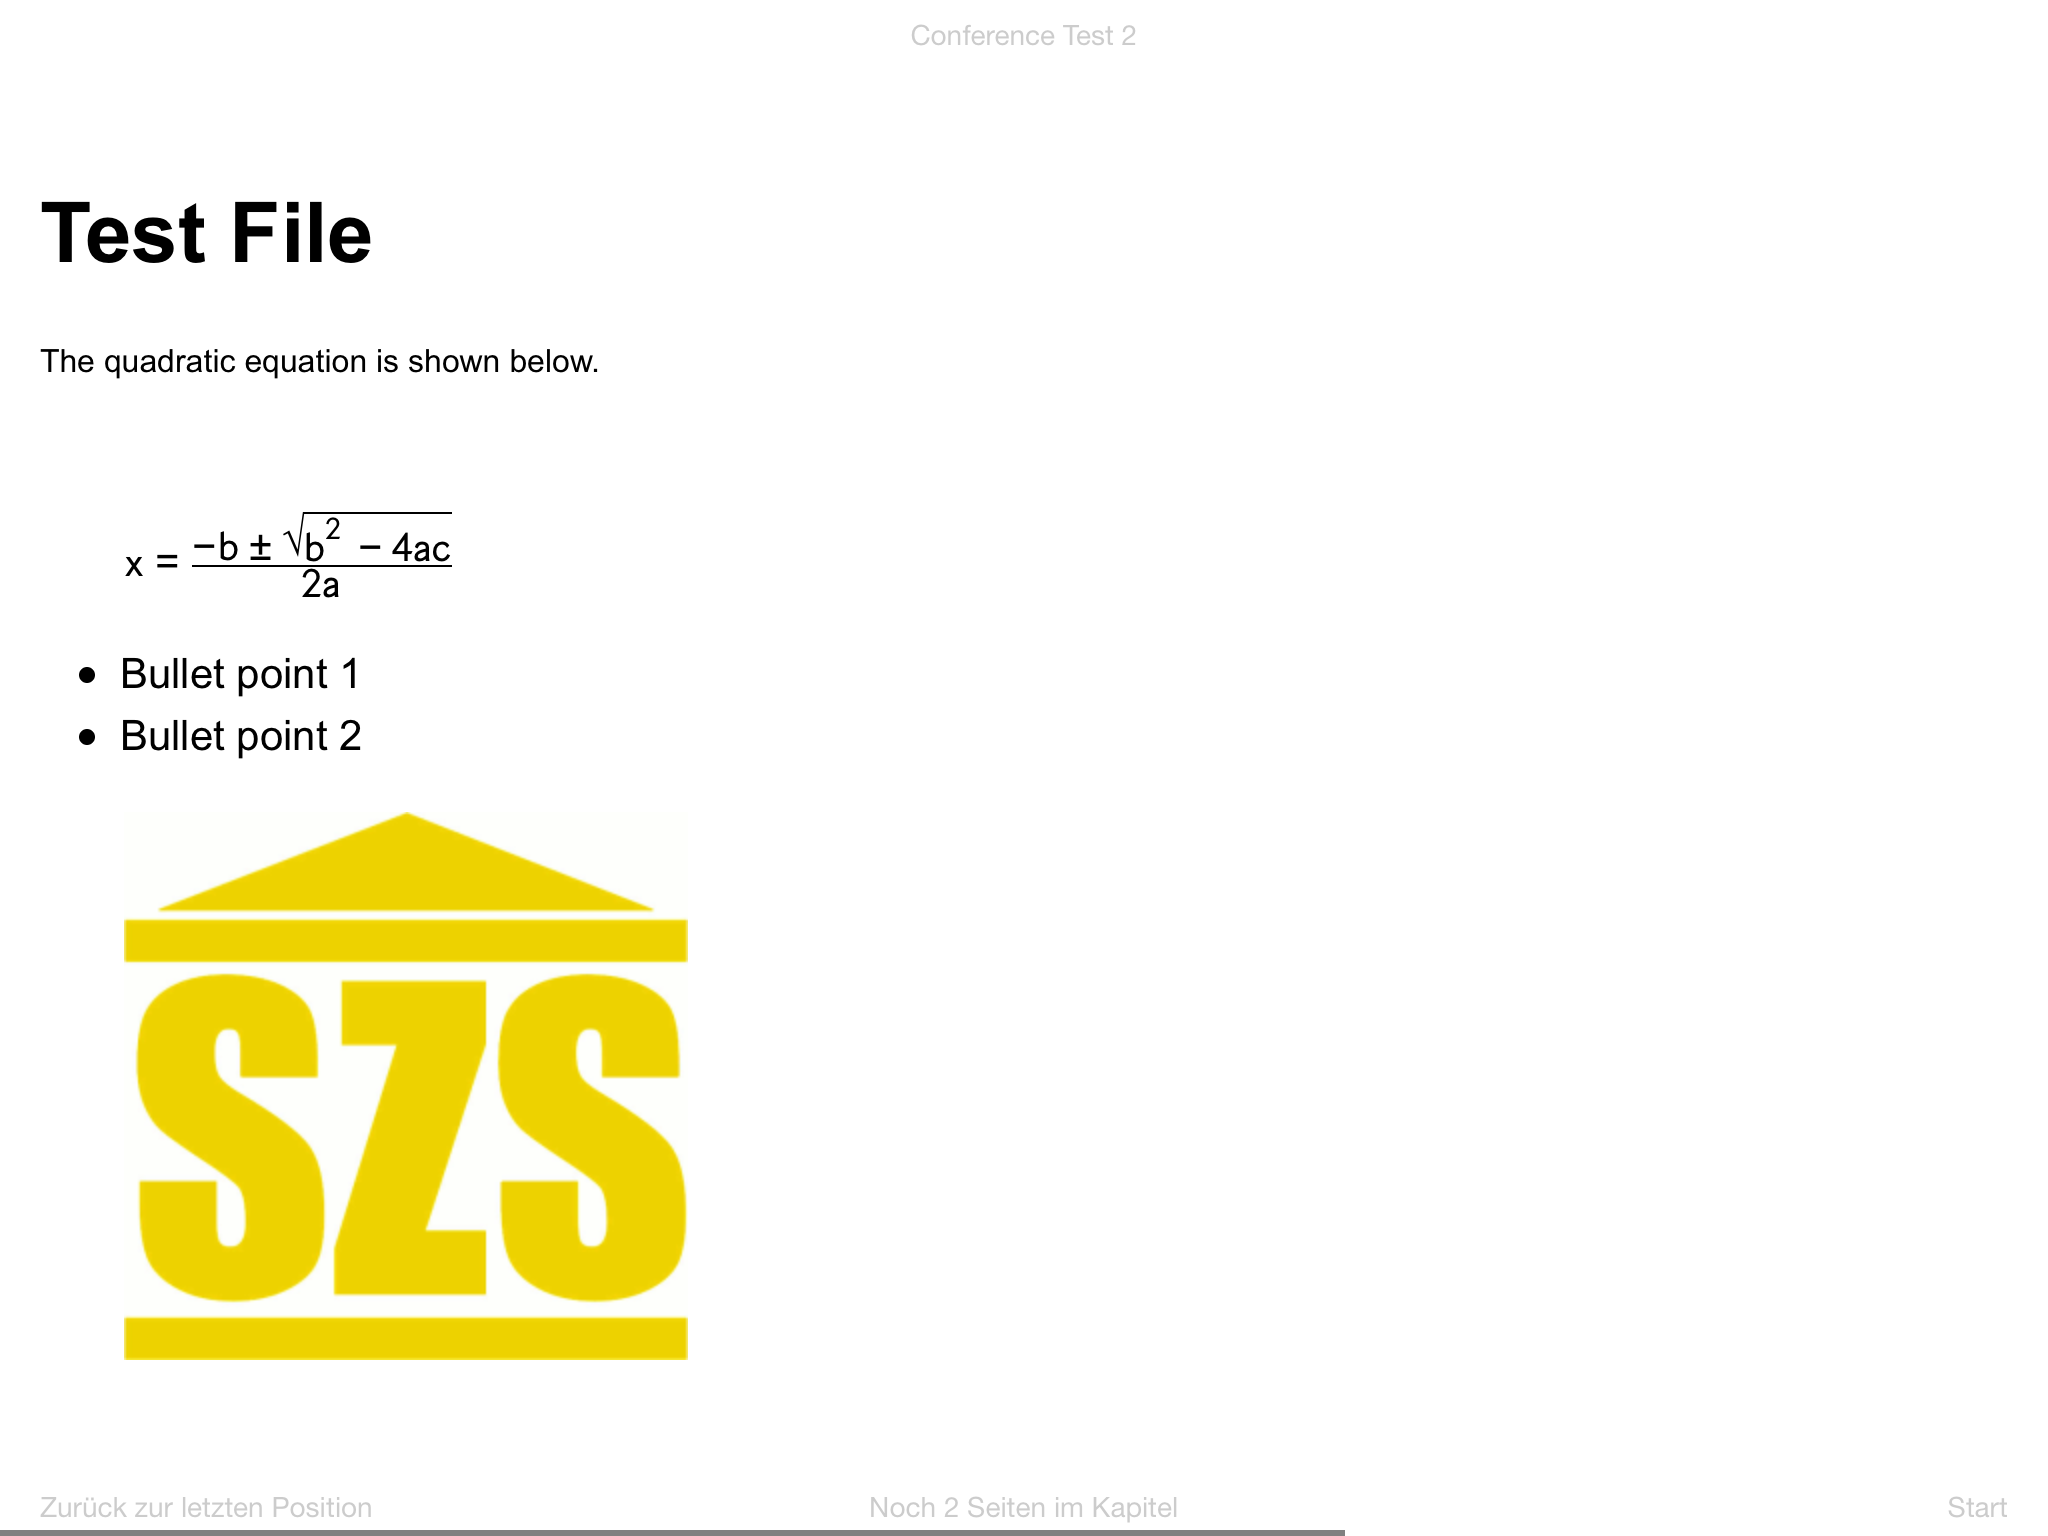
\includegraphics[width=\linewidth*4/5]{figures/MarvinVi.png}}
	\caption{The first half of the visually impaired display style in Marvin}
	\label{fig:marvinVi}
\end{figure}

\begin{comment}
\begin{figure}[H]
	\centering
	\fbox{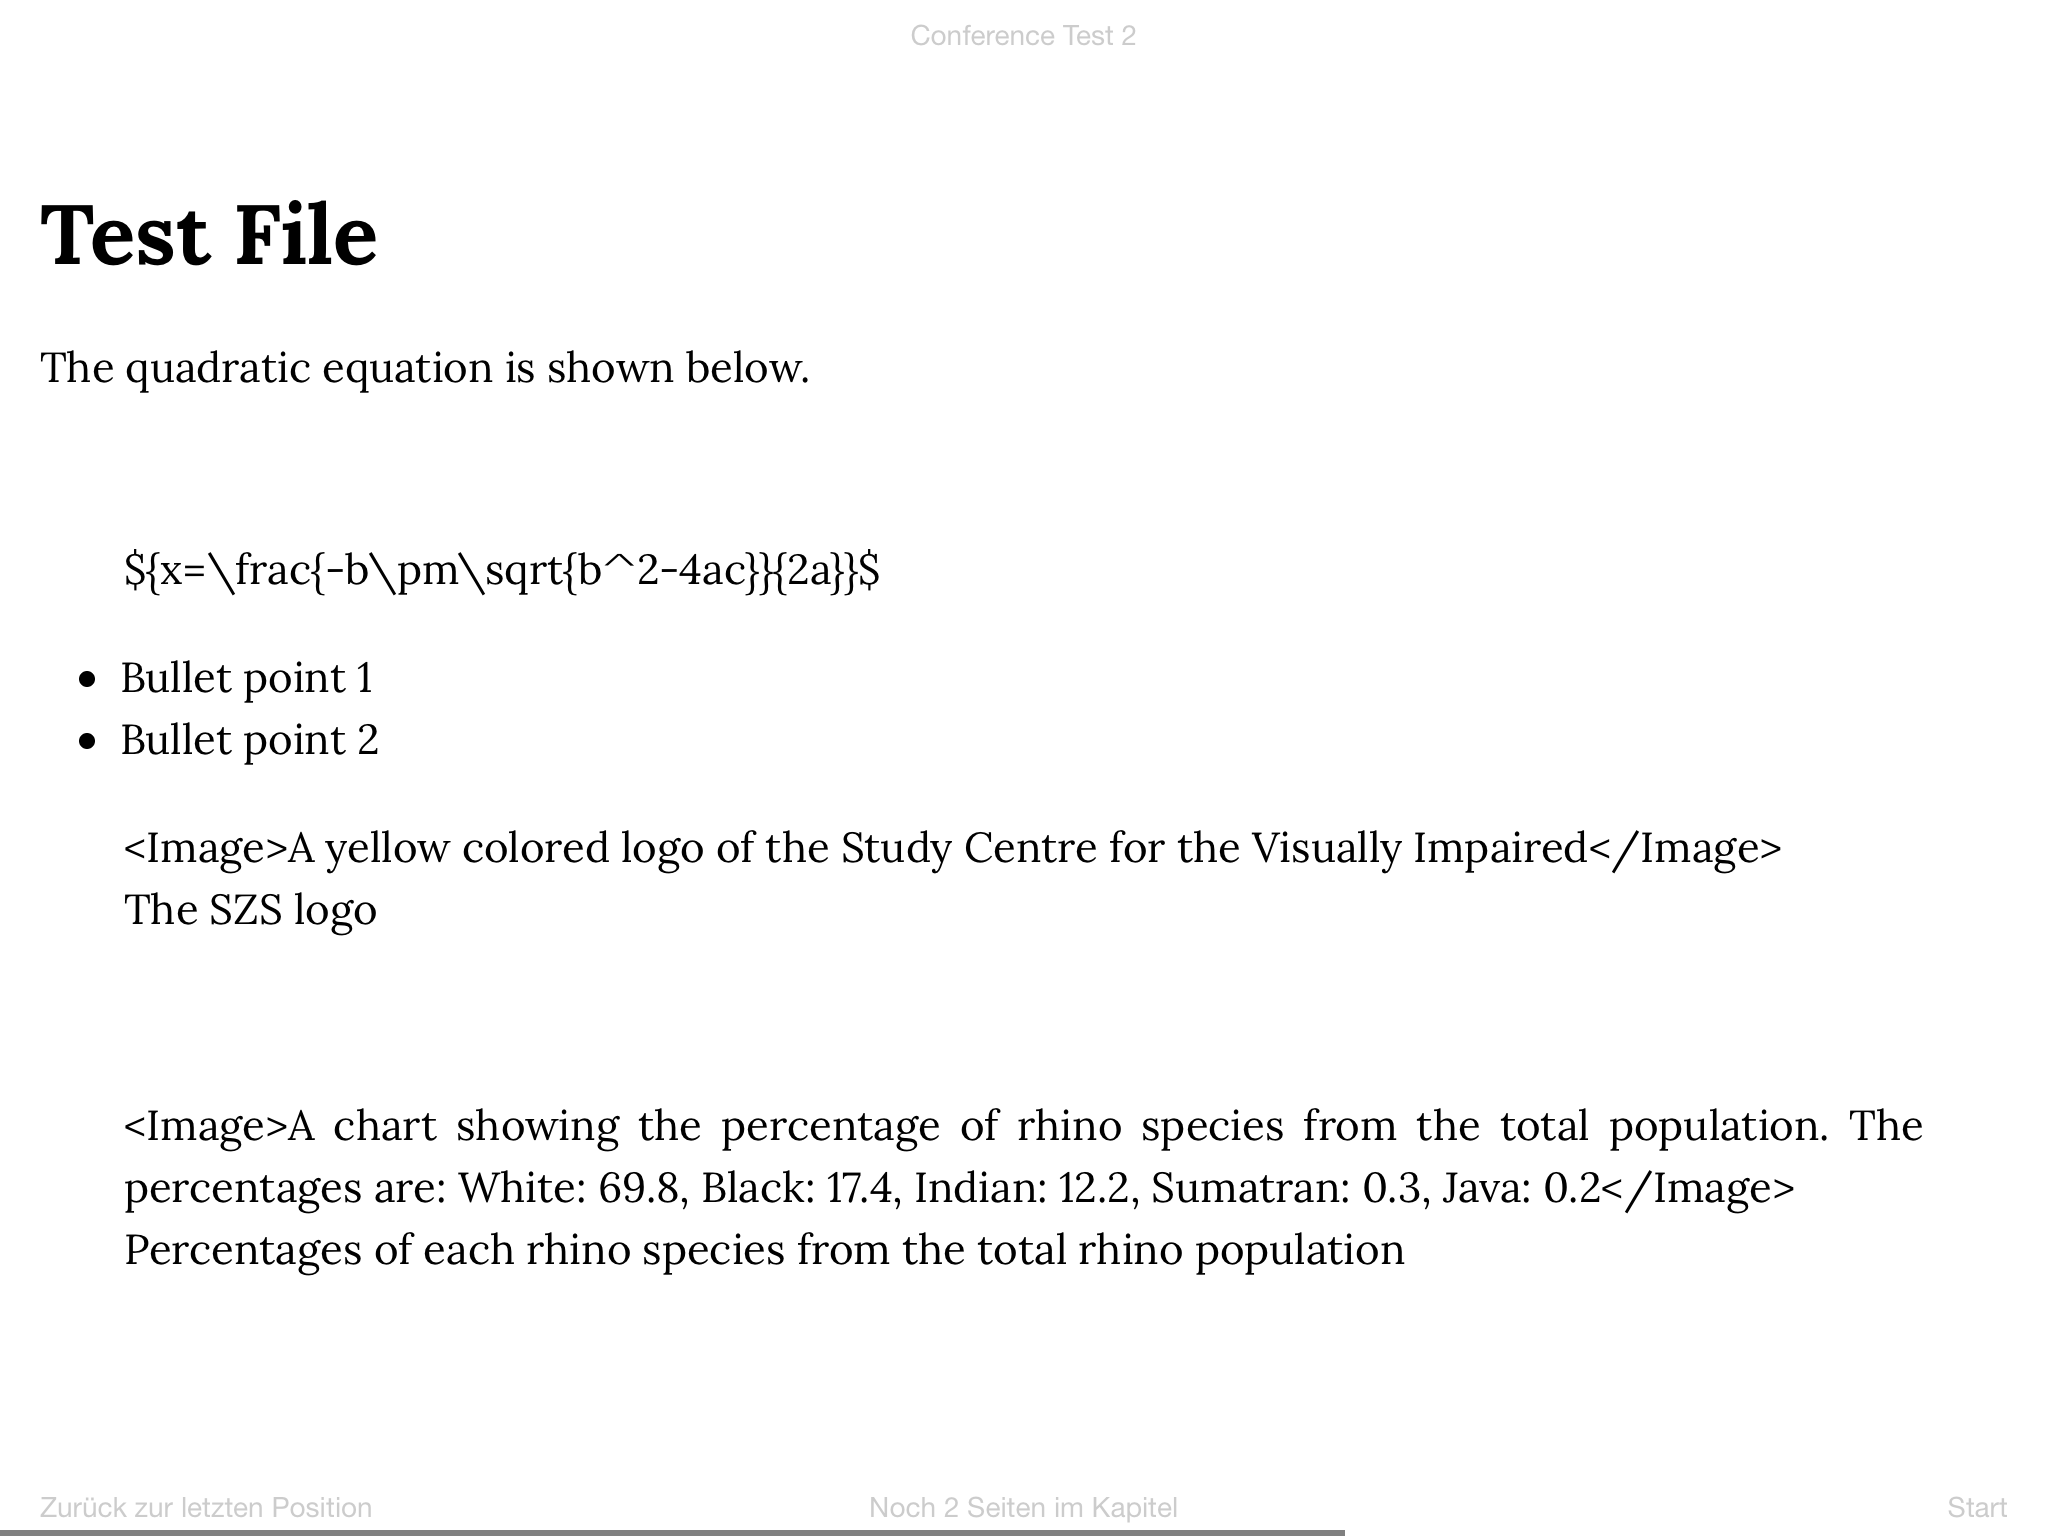
\includegraphics[width=\linewidth*4/5]{figures/MarvinBl.png}}
	\caption{The blind display style in Marvin}
	\label{fig:marvinBl}
\end{figure}
\end{comment}

\subsection{Unusable reading systems}
\subsubsection{iBooks}
iBooks is a E-Book reading system create by Apple for their devices\footnote{https://www.apple.com/ibooks/}. It does not support either one of the switching mechanisms, but can display MathML. Images are not displayed properly, and this likely due to them being in figure elements. The Apple screen reader, VoiceOver, can be used to read EPUB files.

\subsubsection{Yomu}
Yomu EBook Reader on iOS\footnote{https://itunes.apple.com/app/yomu/id562211012} depicts a rendering not seen on other reading systems. In figure \ref{fig:yomu} all elements seem to be displayed correctly. But for some reason the equation appears twice, the first one being a SVG. The SVG is supposed to be hidden and all other reading systems do hide it. It is likely that Yomu does not hide the SVG of an equation which has to included because of the editor in chapter \ref{ch:AccessibleEPUB Editor}. This does not happen to other elements that are hidden the same way. Both the JavaScript and CSS version switching do not work. VoiceOver works with Yomu, and it can even individual elements of a SVG, like the percentages shown in the SVG in the test file.
\begin{figure}[H]
	\centering
	\fbox{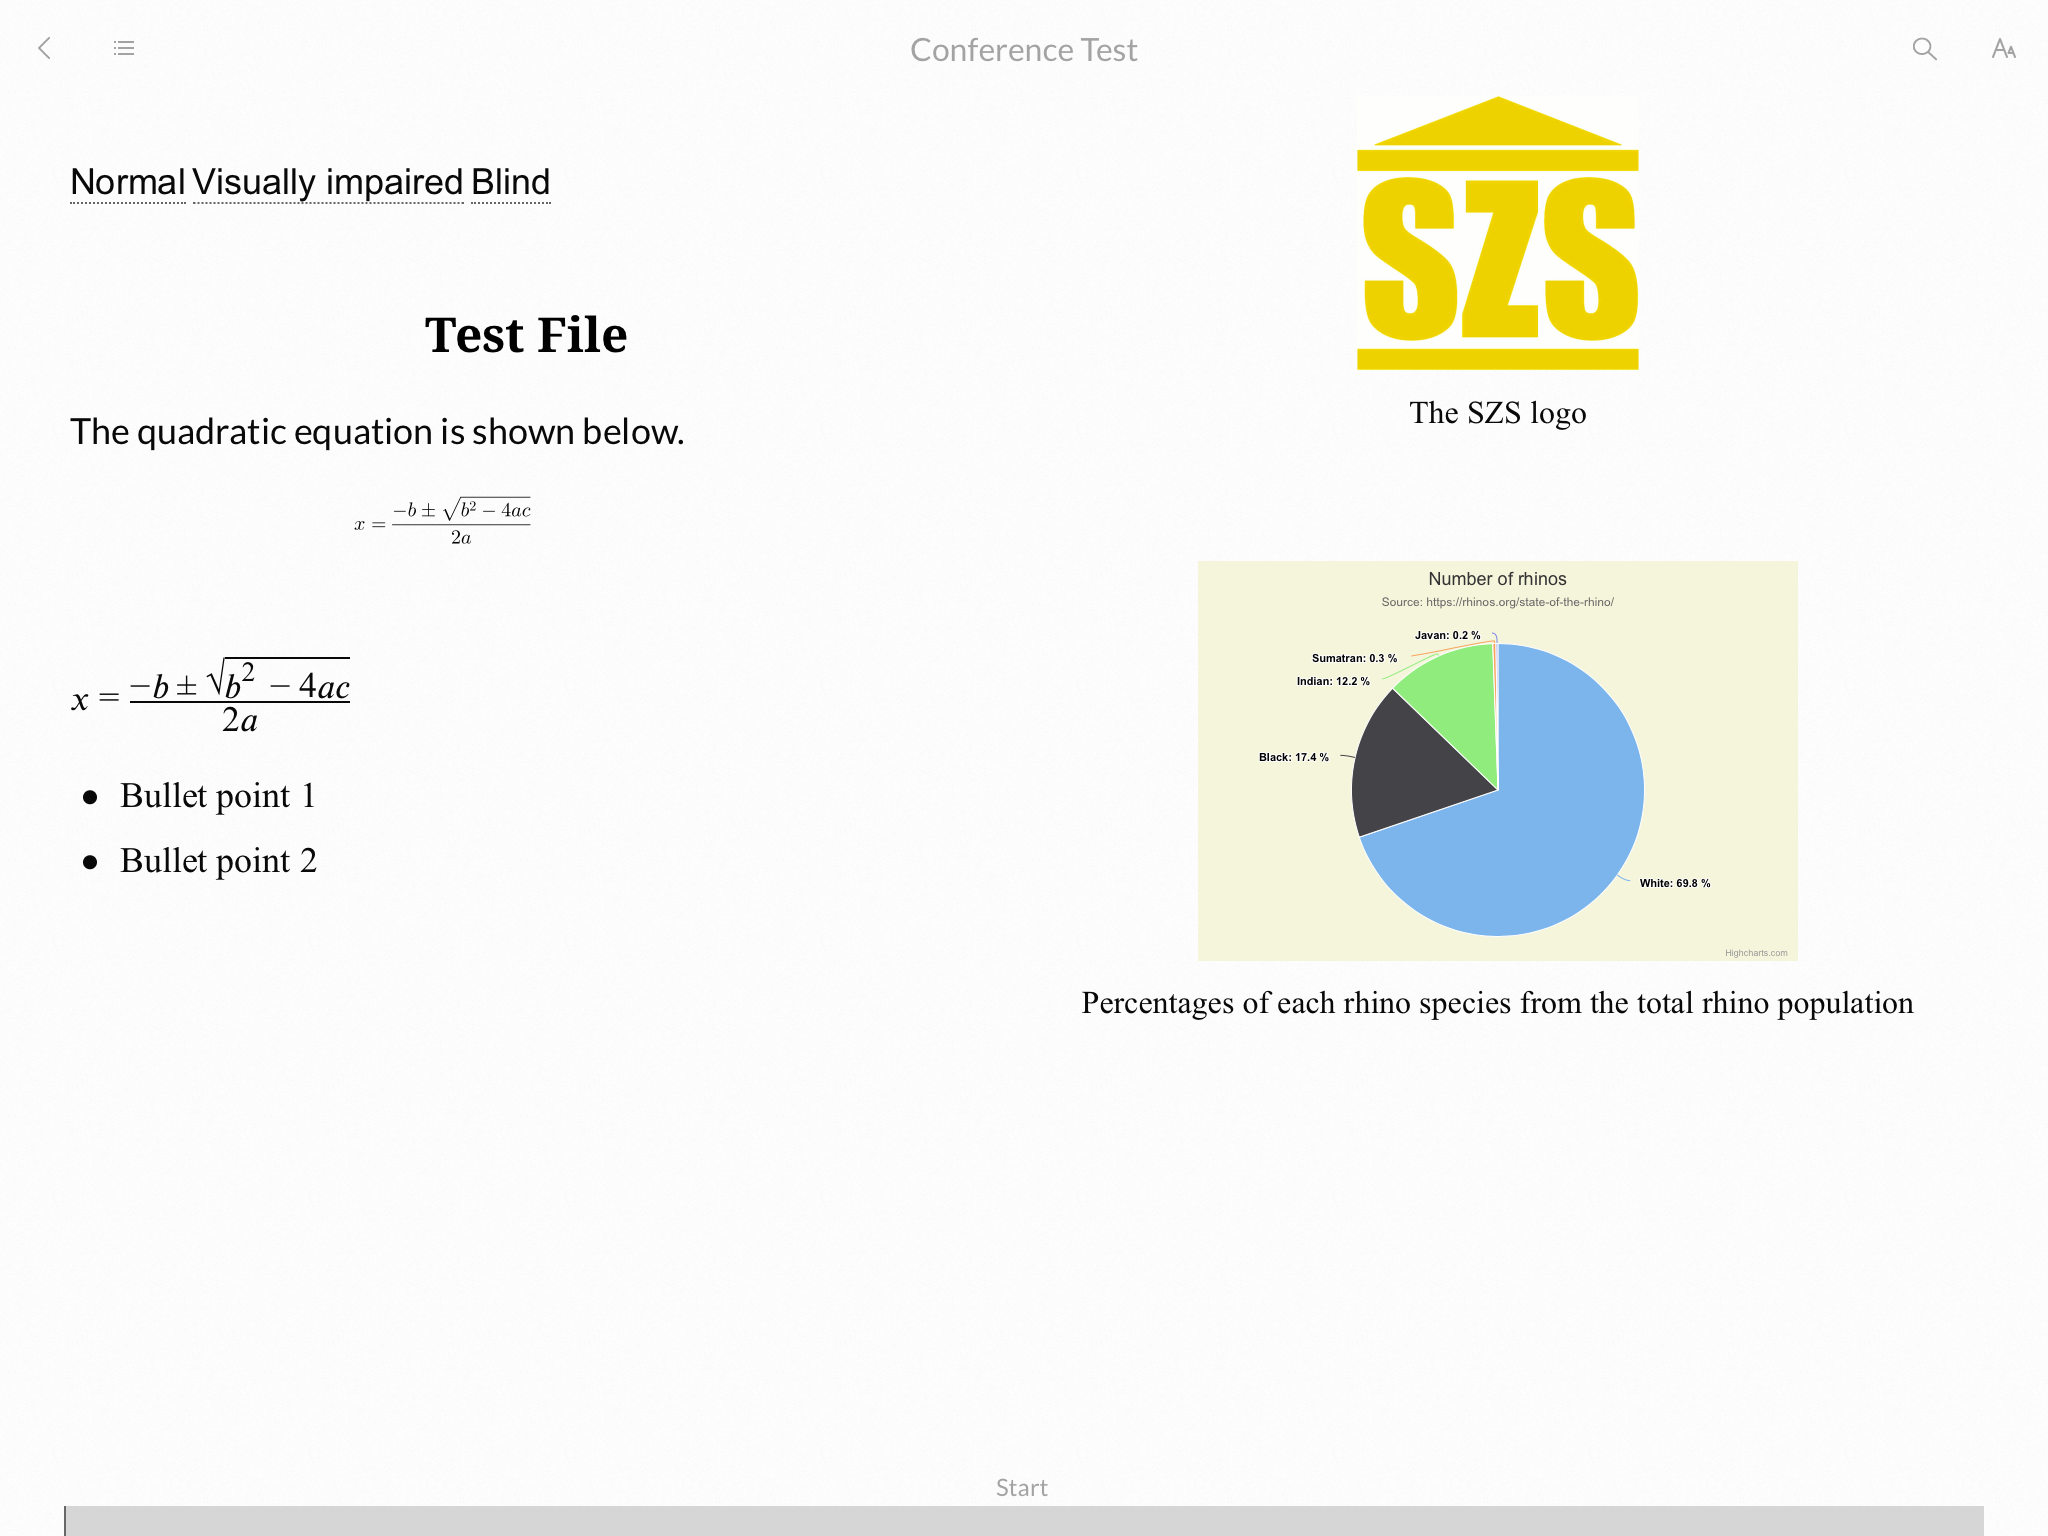
\includegraphics[width=\linewidth*4/5]{figures/Yomu.png}}
	\caption{The CSS file in Yomu}
	\label{fig:yomu}
\end{figure}

\section{Reading systems on Windows}
\subsection{Calibre}
\begin{figure}[H]
	\centering
	\fbox{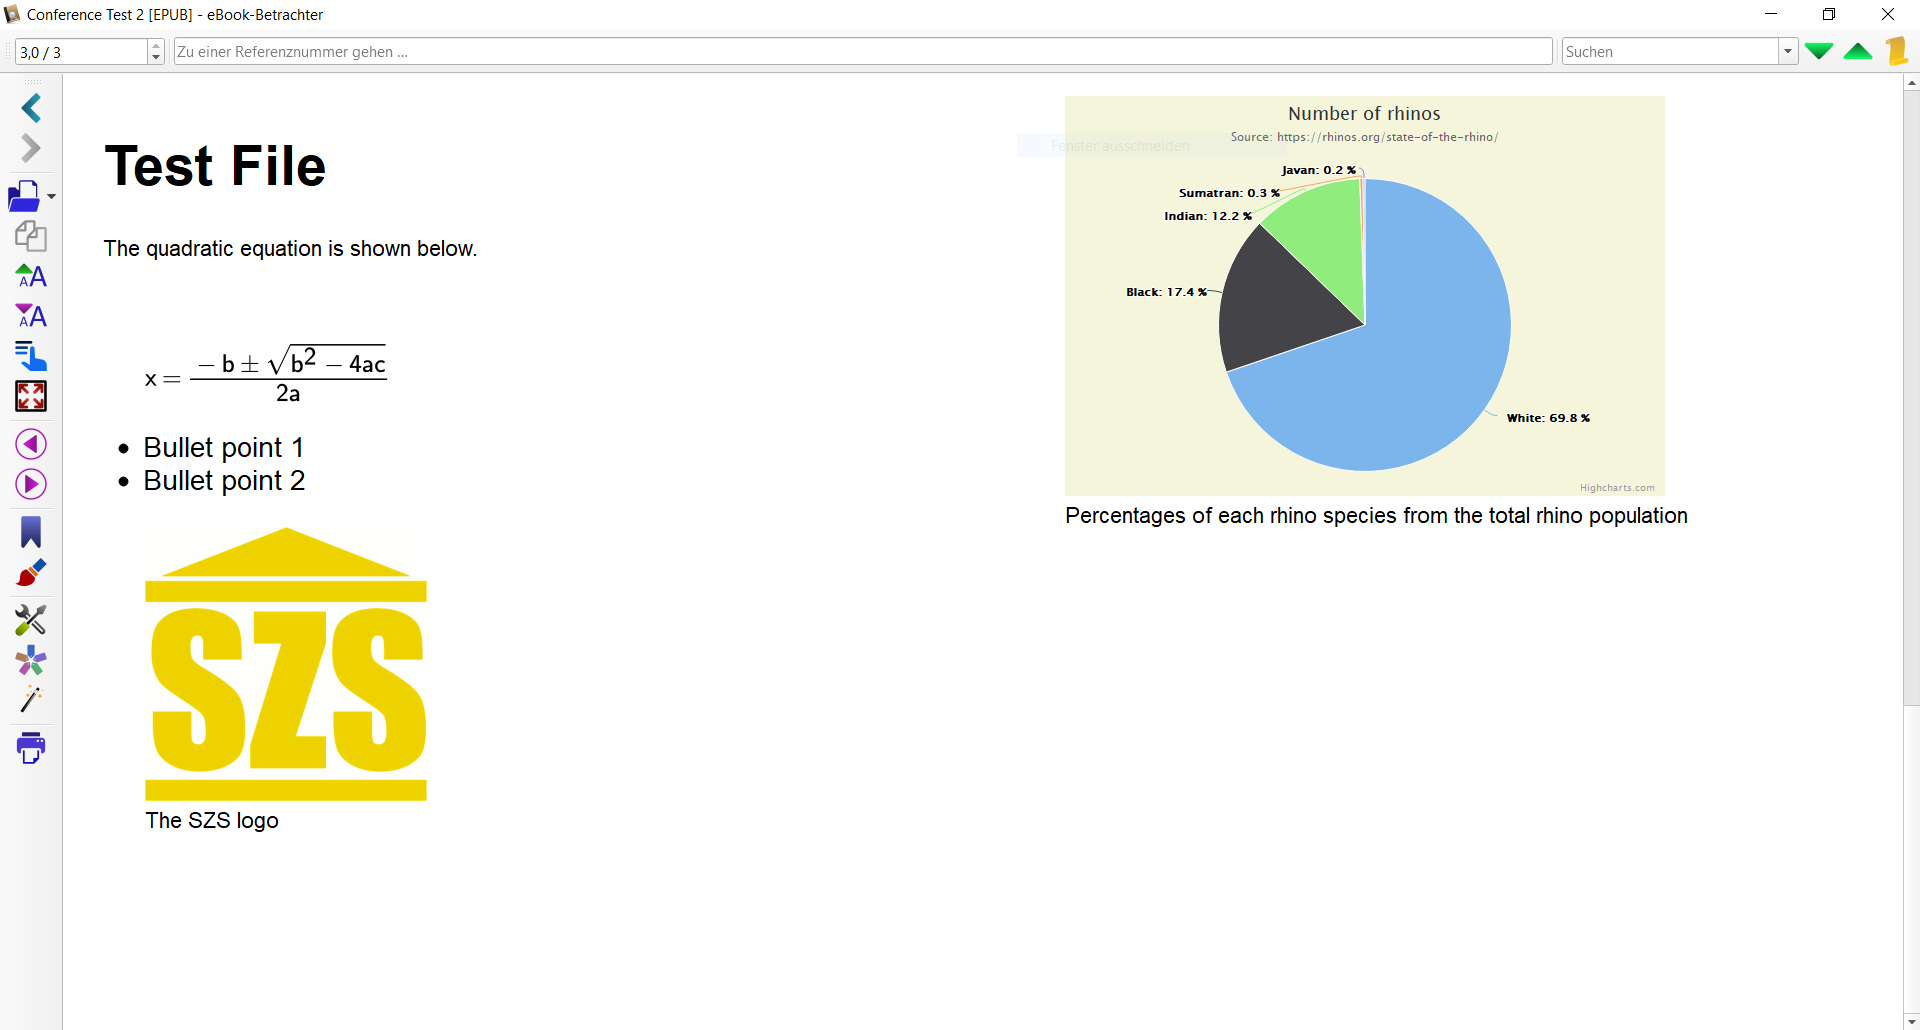
\includegraphics[width=\linewidth]{figures/calibreVi.png}}
	\caption{The visually impaired display style in Calibre}
	\label{fig:calibreVi}
\end{figure}

Calibre is an E-Book management system which is open source\footnote{https://calibre-ebook.com/}. Calibre is the only reading system to support the JavaScript switching. It has session and not local storage, meaning that the display style is remembered until the EPUB is closed. When it is opened again, it goes back to the default display style. As seen in figure \ref{fig:calibreVi} and \ref{fig:calibreBl}, all elements are shown properly, and when the images are hidden in the blind display style, the alternative text is shown properly. The CSS display style is not supported. One major problem with Calibre is that screen readers are not supported, because it is impossible to access figures and text.

\begin{figure}[H]
	\centering
	\fbox{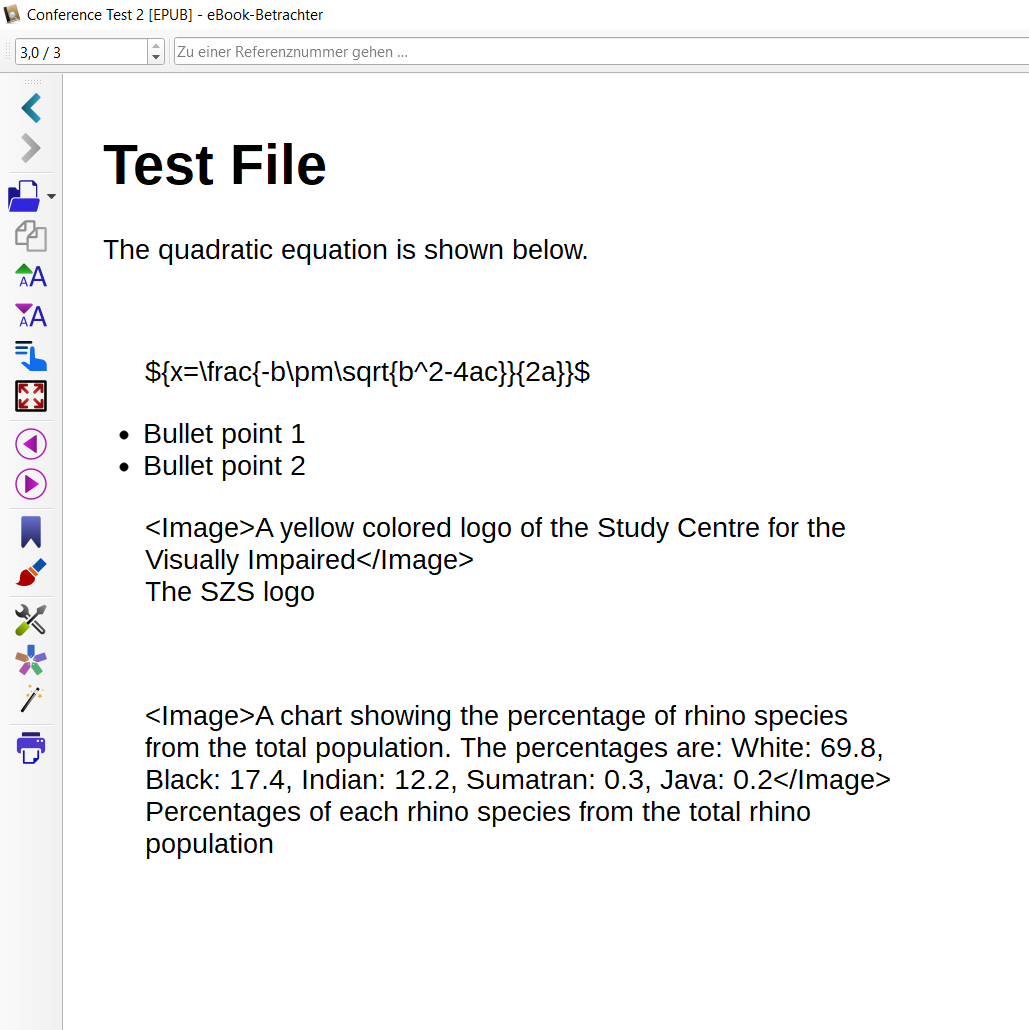
\includegraphics[width=\linewidth*3/5]{figures/calibreBl.png}}
	\caption{The blind display style in Calibre}
	\label{fig:calibreBl}
\end{figure}

\subsection{Readium}

\begin{figure}[H]
	\centering
	\fbox{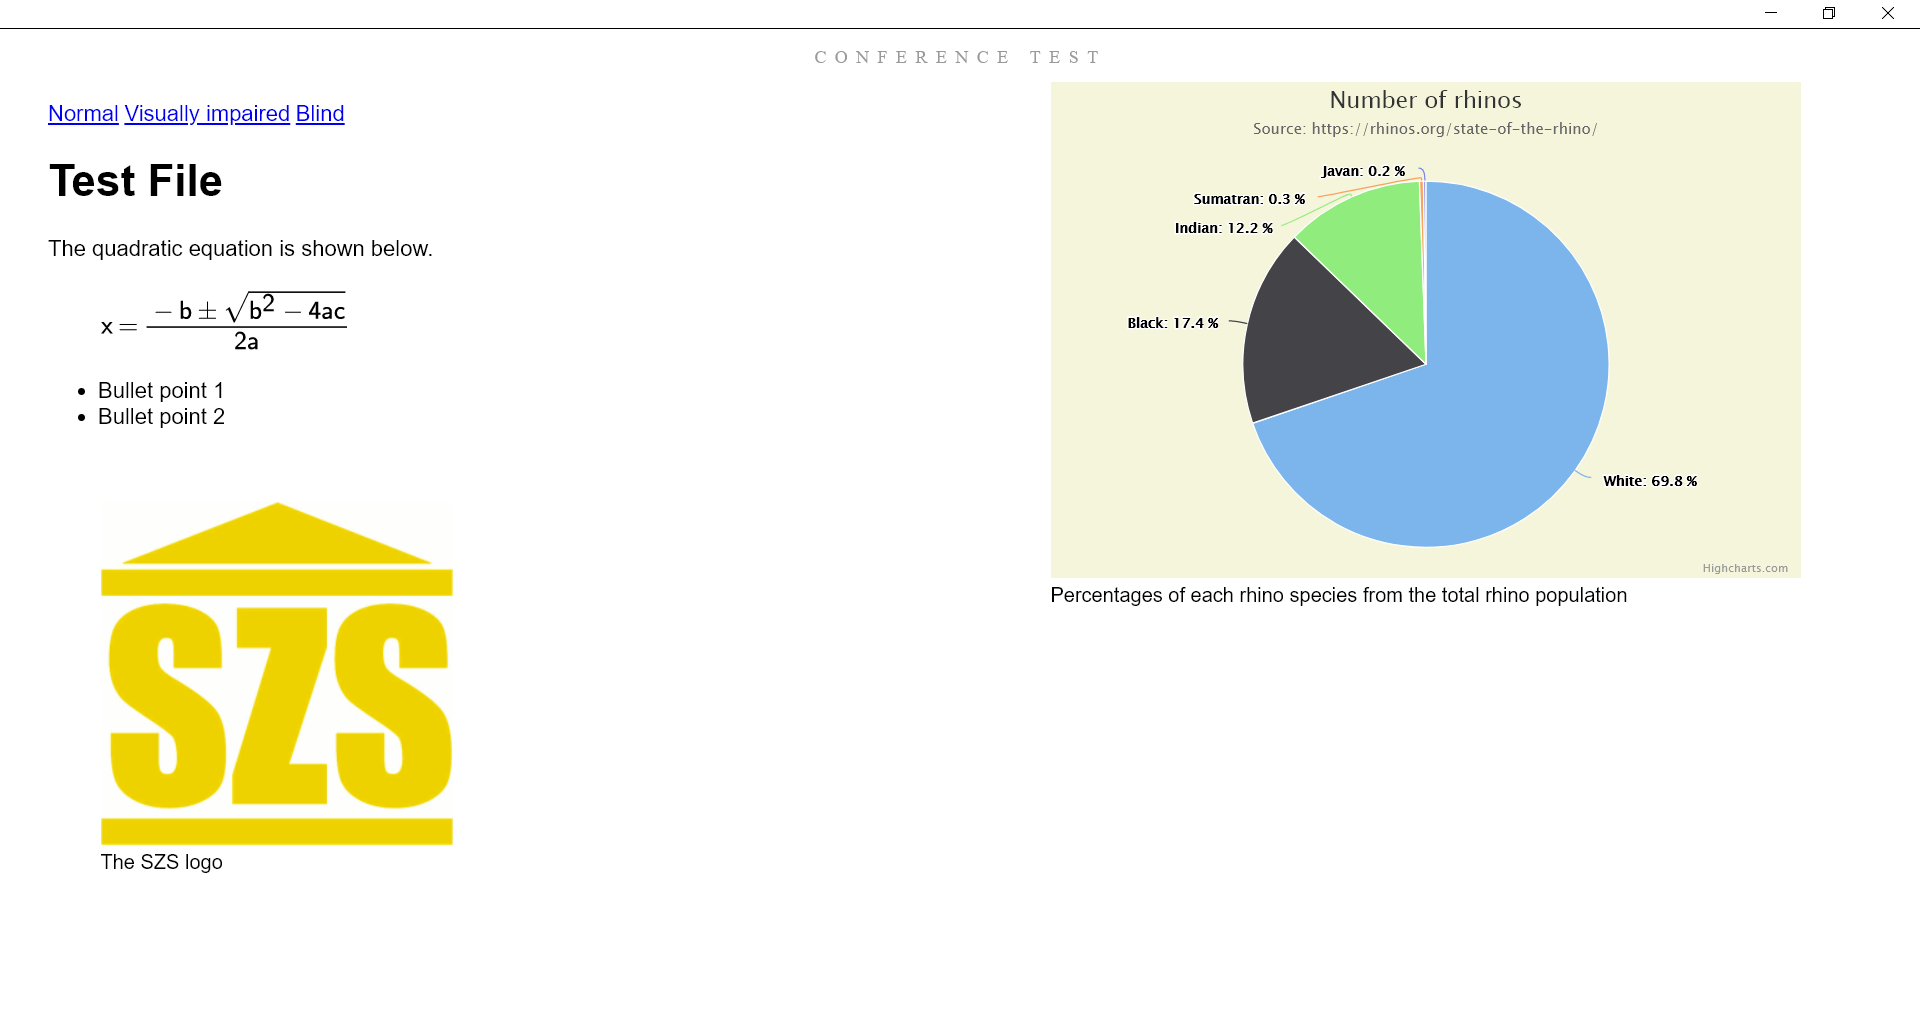
\includegraphics[width=\linewidth]{figures/ReadiumVi.png}}
	\caption{The visually impaired display style in Readium}
	\label{fig:ReadiumVi}
\end{figure}
Readium began as a project of the IDPF as an open source application to create reading systems which follow the newest EPUB standards\footnote{http://readium.org/about/faq}. As such, it supports many of the new features. As shown in figures \ref{fig:ReadiumVi} and \ref{fig:ReadiumBl}, both the visually impaired and blind display style of the CSS standard are shown as intended. The JavaScript standard does not work. Furthermore, it supports screen readers and everything is identified correctly. However, there still is one issue. While testing several CSS EPUB documents, the switching in the short ones did not function properly. In the preview browser in Accessible EPUB and when the individual XHTML files were opened in web browsers the behaved correctly.


\begin{figure}[H]
	\centering
	\fbox{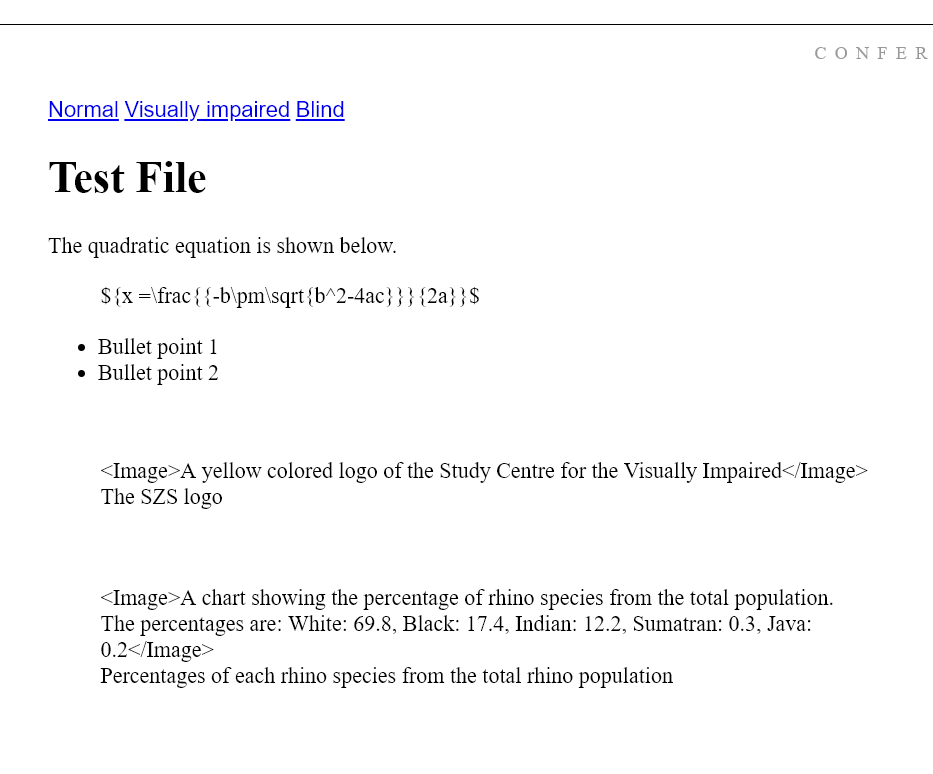
\includegraphics[width=\linewidth]{figures/ReadiumBl.png}}
	\caption{The blind display style in Readium}
	\label{fig:ReadiumBl}
\end{figure}


\subsection{Unusable reading systems}
\subsubsection{Bluefire Reader}
Figure \ref{fig:Bluefire} of the Bluefire Reader\footnote{http://www.bluefirereader.com/bluefire-reader.html} is very similar to figure \ref{fig:tolino} of the Tolino app. They don't show the images and cannot display MathML properly. Both CSS and JavaScript switching do not work. Screen readers can also not read the content of the document.
\begin{figure}[H]
	\centering
	\fbox{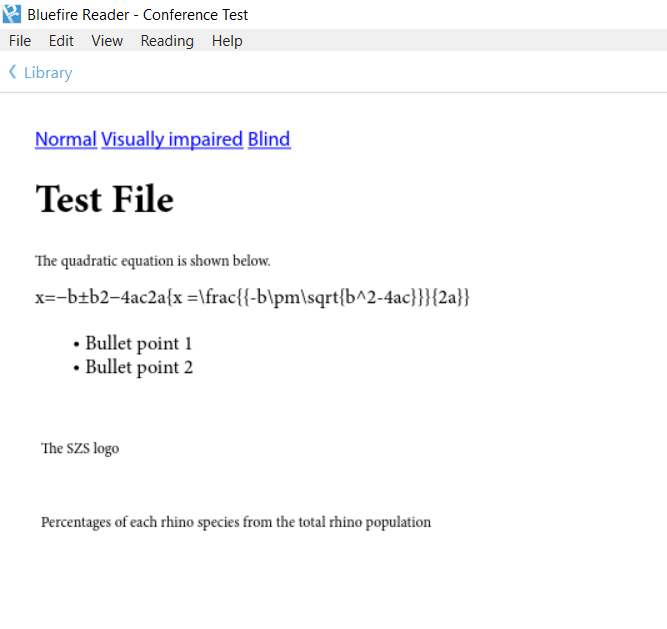
\includegraphics[width=\linewidth*3/5]{figures/Bluefire.png}}
	\caption{The CSS file in Bluefire Reader}
	\label{fig:Bluefire}
\end{figure}
\subsubsection{Icecream Ebook Reader}
Figure \ref{fig:Icecream} shows the CSS test file open in Icecream Ebook Reader\footnote{https://icecreamapps.com/Ebook-Reader/}. While MathML is not displayed properly the SVG and PNG are shown correctly. The switching mechanism does not work either with CSS or JavaScript and there is no screen reader support.
\begin{figure}[H]
	\centering
	\fbox{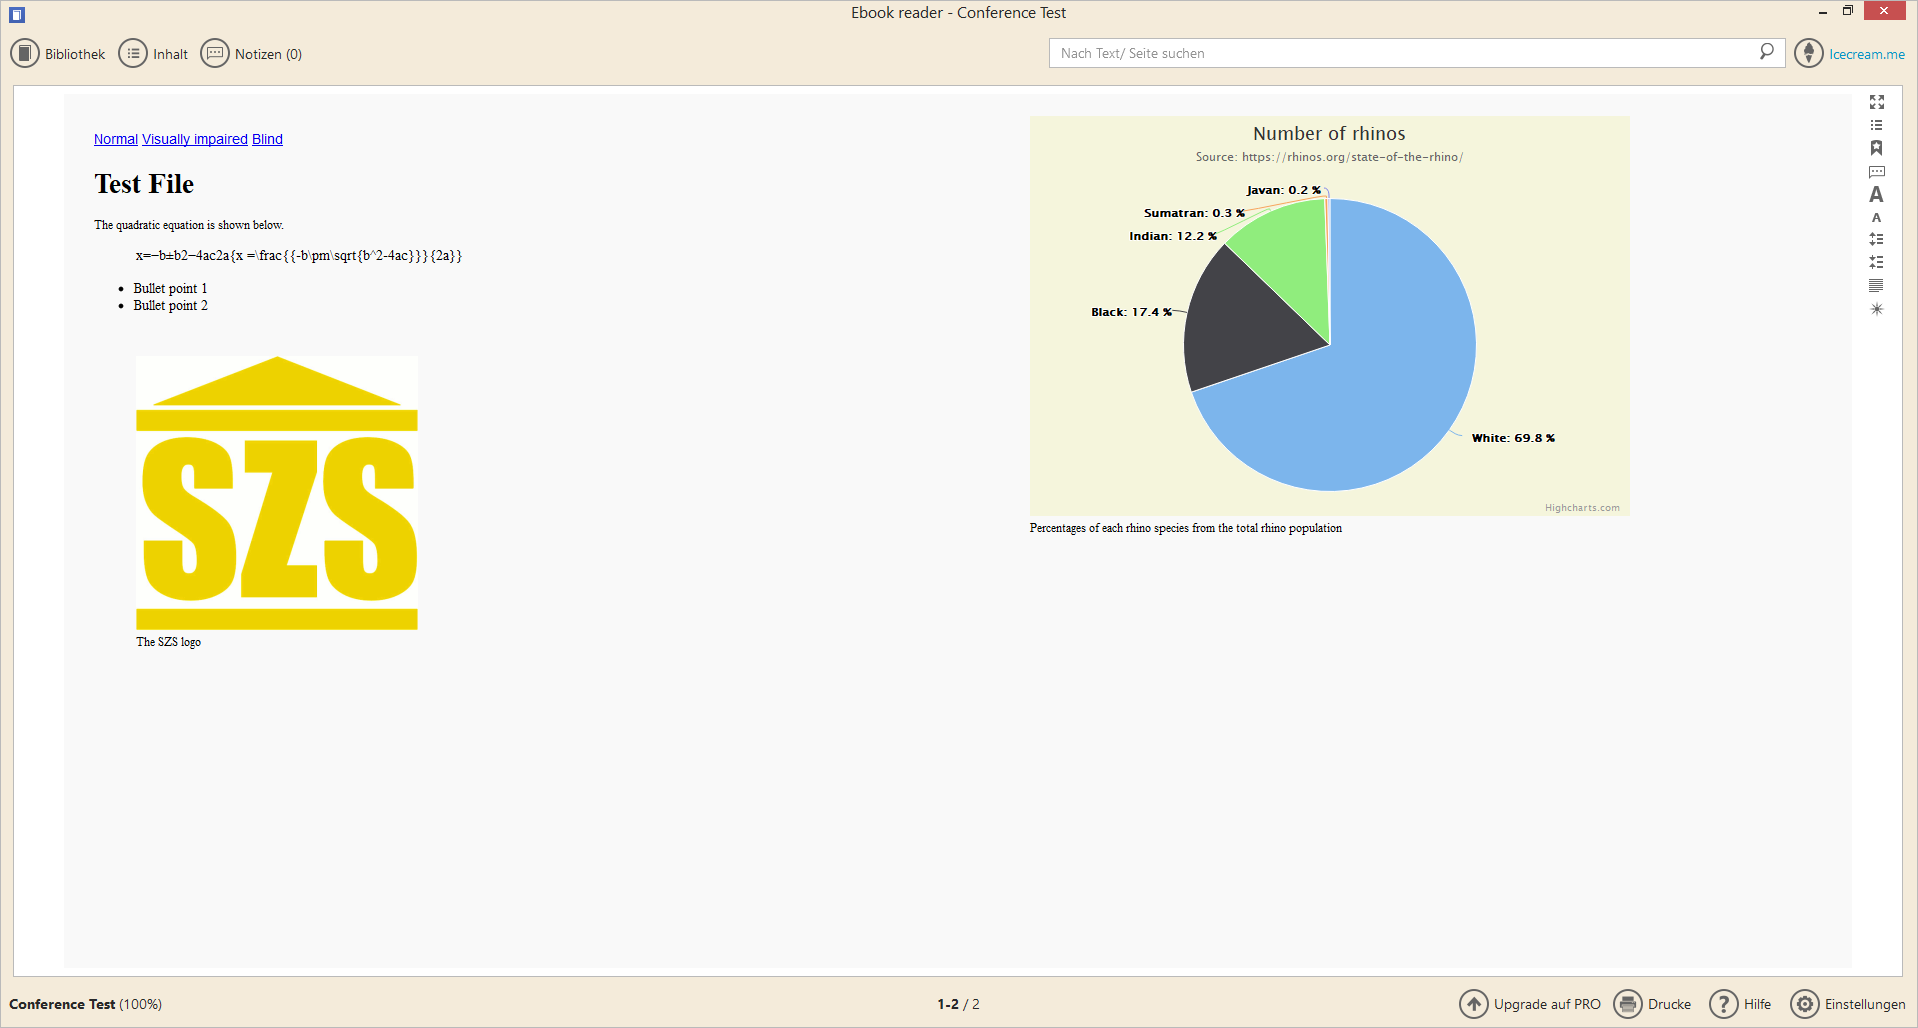
\includegraphics[width=\linewidth]{figures/Icecream.png}}
		\caption{The CSS file in Icecream Ebook Reader}
	\label{fig:Icecream}
\end{figure}

\subsubsection{AZARDI}
AZARDI Desktop\footnote{http://azardi.infogridpacific.com/} is a E-Book reader recommended by the DAISY consortium \cite{daisyAZARDI} as supports accessibility and it works with the JAWS screen reader. Furthermore, as seen in figure \ref{fig:AZARDI}, it displays most of the content correctly, including MathML. The elements it does not display correctly are the links. They are shown as normal text and it is not indicated that they can be clicked. The switching mechanism does not work in both CSS and JavaScript.
\begin{figure}[H]
	\centering
	\fbox{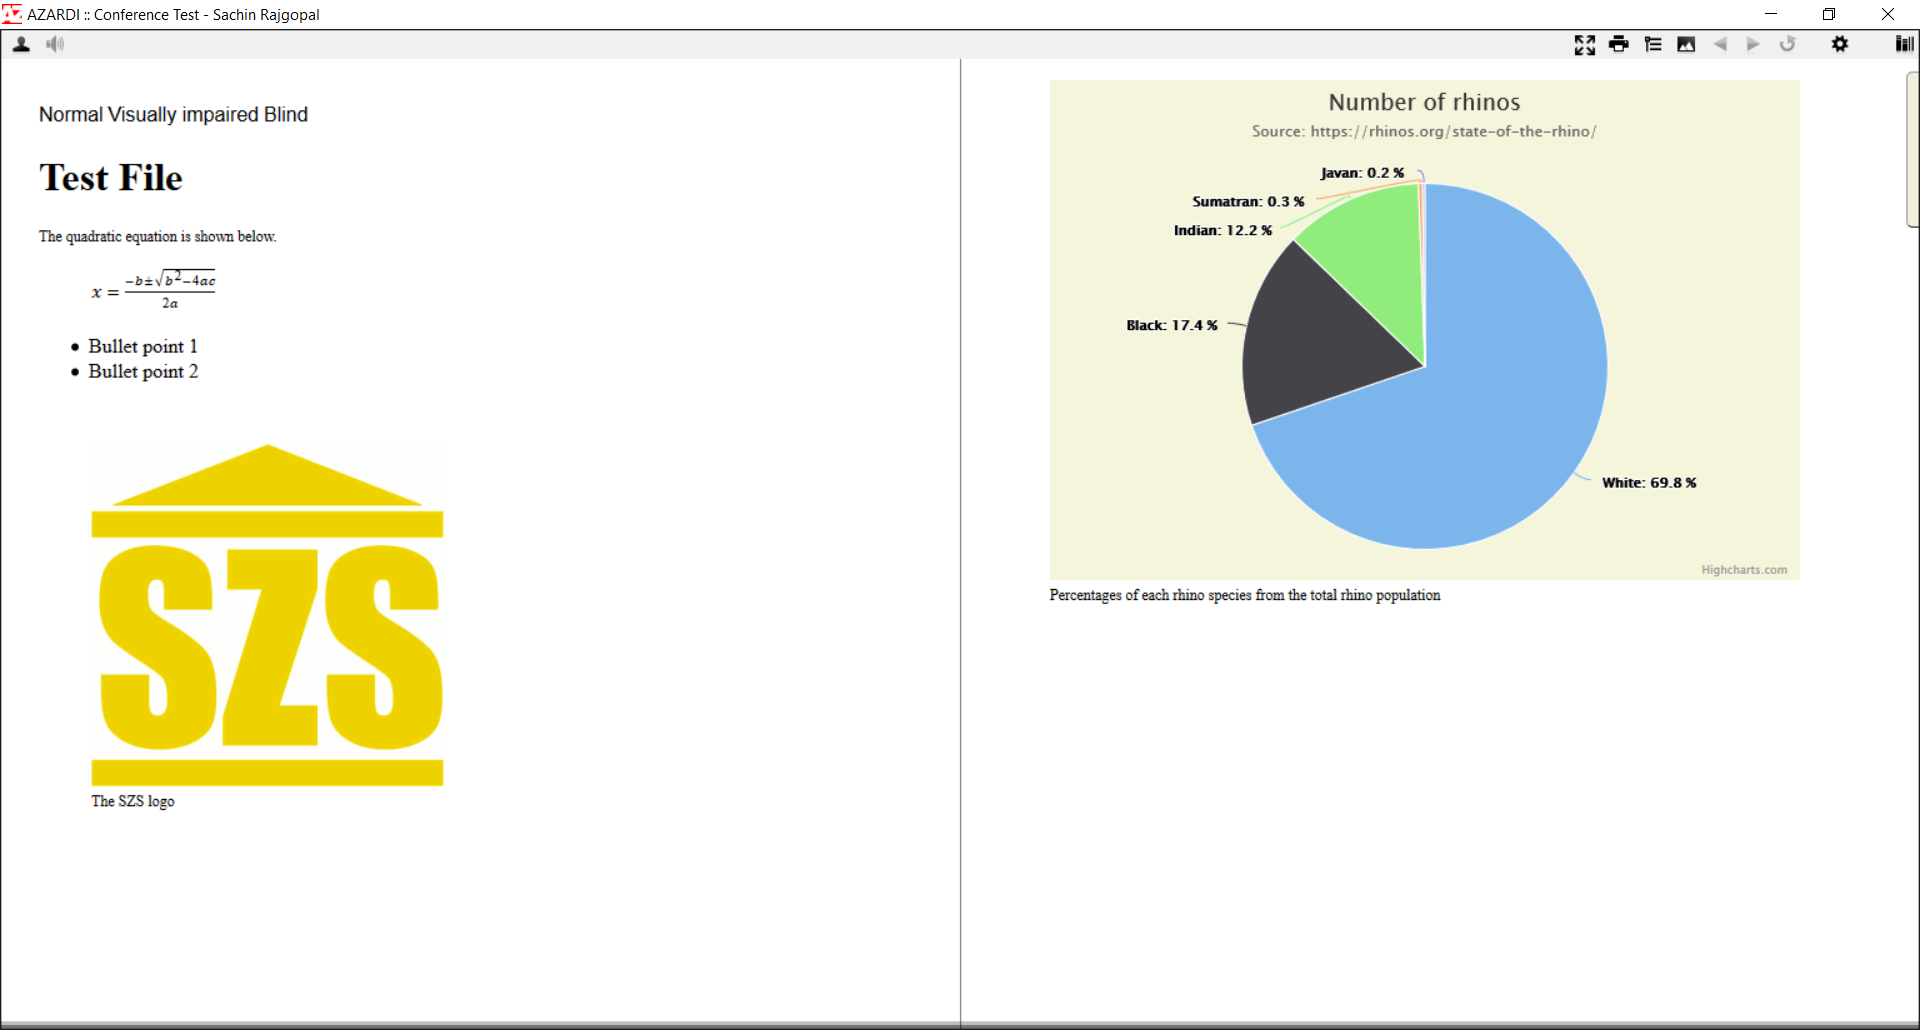
\includegraphics[width=\linewidth]{figures/Azardi.png}}
	\caption{The CSS file in AZARDI}
	\label{fig:AZARDI}
\end{figure}

\subsubsection{Adobe Digital Editions}
\begin{figure}[H]
	\centering
	\fbox{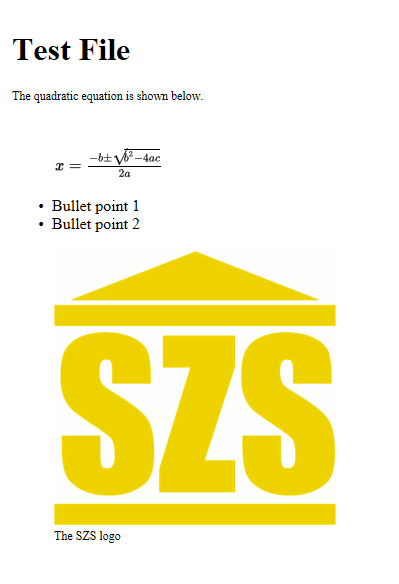
\includegraphics[width=\linewidth/3]{figures/AdobeDigitalEditions.png}}
	\caption{The JavaScript file in Adobe Digital Editions}
	\label{fig:adobeDigital}
\end{figure}

In figure \ref{fig:adobeDigital} the first half of the content is shown. While the equation and the images were displayed correctly, the equation has not been rendered well. The root symbol is poorly formatted and it is not properly spaced. Screen readers do not work.

\section{Discussion: what do developers have to do?}

The EPUB 3 specification \cite{EPUBspecs} was recommended on the 11th of October 2011. More than 6 years later, most of the EPUB reading systems do not support the new features, such as MathML and CSS 3. Developers have to start supporting the new features as soon as possible. The CSS standard only works in Reasily and Readium, while the JavaScript standard only works in Calibre on Windows 10. JavaScript is optional so developers don't have to necessarily support that standard, but CSS is part of the EPUB specification. It is important that the new CSS features will be supported soon, so that the CSS standard functions properly. Even Readium which was originally created by the IDPF does not support the CSS perfectly. It seems like EPUB 3 will remain the standard for a longer period of time as EPUB 3.1 specification was just recommended on the 5th of January 2017 and it was just a small update. So developers of EPUB reading systems can be assured that the EPUB 3 specification won't be completely overworked in the foreseeable future and having some security for the future. 

\section{Conclusion}
\begin{table}
	\centering
	\caption{Features supported by several EPUB reading systems}
	\begin{tabular}{| c | c | c | c | c |}
		\hline
		& CSS & JavaScript & MathML & Screen reader \\ \hline
		\textbf{Reasily} & \cmark & \xmark & \cmark & \cmark \\  \hline
		Tolino & \xmark & \xmark & \xmark & \xmark \\ \hline
		Gitden & \xmark & \xmark & \cmark & \cmark \\ \hline
		FBReader & \xmark & \xmark & \xmark & \xmark \\ \hline
		UB Reader & \xmark & \xmark & \xmark & \xmark \\ \hline
		
		\textbf{Marvin} & \xmark & \cmark & \cmark & \cmark \\ \hline
		iBooks & \xmark & \xmark & \cmark & \cmark \\ \hline
		Yomu & \xmark & \xmark & \cmark & \cmark \\ \hline
		
		\textbf{Calibre} & \xmark & \cmark & \cmark & \xmark \\ \hline
		\textbf{Readium} & \cmark & \xmark & \cmark & \cmark \\ \hline		
		Bluefire Reader & \xmark & \xmark & \xmark & \xmark \\ \hline
		Icecream Ebook Reader & \xmark & \xmark & \xmark & \xmark \\ \hline
		AZARDI & \xmark & \xmark & \cmark & \cmark \\ \hline		
		Adobe Digital Editions & \xmark & \xmark & \cmark & \cmark \\ \hline
		
	\end{tabular}
	\label{fig:table}
\end{table}

As seen figure \ref{fig:table}, many EPUB reading systems do not even process MathML correctly, and many were chosen due to them listing MathML support as a feature. Even fewer can use the switching mechanism with either version. A few of them do work though. On Android Reasily is the recommended app as it works well with the CSS version. Marvin can display with JavaScript version correctly in iOS. On Windows 10 Calibre works the best with the JavaScript version, but screen readers do not identify the content area. Readium works well with CSS version, but there are still some usability issues where short files do not switch display styles. It is, however, still the best option on Windows as it screen readers can work with it.